% SPDX-License-Identifier: CC-BY-SA-4.0
%
% Copyright (c) 2020 Philipp Le
%
% Except where otherwise noted, this work is licensed under a
% Creative Commons Attribution-ShareAlike 4.0 License.
%
% Please find the full copy of the licence at:
% https://creativecommons.org/licenses/by-sa/4.0/legalcode

\chapter{Modulation and Mixing}

\begin{refsection}
	
The task of a communication system is transmitting information.

Example: Voice transmission
\begin{itemize}
	\item Voice has a spectrum from about \SI{20}{Hz} to \SI{20}{kHz}
	\item It is not feasible to transmit the spectrum directly as electromagnetic waves.
	\item The electromagnetic spectrum must be shared with myriads of other users.
	\item So, the voice is shifted to a higher frequency, for example, \SI{144.3}{MHz}.
	\item The voice is \emph{modulated} on this \emph{carrier} of \SI{144.3}{MHz}.
	\item The voice is then located from about \SI{144.28}{MHz} to \SI{144.32}{MHz}.
\end{itemize}

\begin{definition}{Modulation}
	\index{modulation} \textbf{Modulation} is the process of altering a signal -- the \index{carrier} \textbf{carrier} -- so that it contains the information to be transmitted.
\end{definition}

\begin{definition}{Demodulation}
	\index{demodulation} \textbf{Demodulation} is the inverse process of modulation. The information is extracted from the carrier.
\end{definition}

In the previous example, the voice was the information-carrying signal. This can be transferred to any kind of information. In this chapter, we will discuss techniques to modulate data on carriers which can be transmitted over wired and wireless channels.

\todo{Block diagram modulator}

\section{Modulation in The Time and Frequency Domain}

Generally, the carrier is a \emph{monochromatic} signal, i.e., it is a sinusoidal function. A sinusoidal function has three parameters: (angular) frequency $\omega_C$, phase $\varphi_C$ and amplitude $\hat{X}_C$.
\begin{equation}
	x_C(t) = \hat{X}_C \cos\left(\omega_C t + \varphi_C\right)
	\label{eq:ch05:carrier_timedomain}
\end{equation}
The frequency is fixed to the carrier frequency. The other two parameters can be altered and the information can be modulated into them.

There are two classes of modulation:
\begin{itemize}
	\item \textbf{Amplitude modulation} The amplitude of the carrier is altered.
	\begin{equation}
		x_{S,AM}(t) = f_{\hat{X}}(t) \cos\left(\omega_C t + \varphi_C\right)
	\end{equation}
	\item \textbf{Phase modulation} The phase of the carrier is altered.
	\begin{equation}
		x_{S,PM}(t) = \hat{X}_C \cos\left(\omega_C t + f_{\varphi}(t)\right)
	\end{equation}
\end{itemize}

This section covers basic modulation techniques of analogue signals.
\begin{itemize}
	\item The considerations are explanatory and are extended to digital signals in the following section.
	\item This section shall offer an understanding of how modulation works in general (for both analogue and digital signals).
	\item A digital signal must be converted to an analogue signal in order to physically exists. It can then be modulated onto a carrier and transmitted as an electromagnetic wave.
\end{itemize}

\subsection{Amplitude Modulation}

The \index{amplitude modulation} \textbf{\ac{AM}} is the alteration of the carrier's amplitude.

\begin{attention}
	By now, all signals are real, because the technical realization is considered. Physical signals must always be real.
\end{attention}

The carrier is a mono-chromatic signal:
\begin{equation}
	x_C(t) = \hat{X}_C \cdot \cos\left(2\pi f_C + \varphi_C\right)
\end{equation}
where
\begin{itemize}
	\item $\hat{X}_C$ is the amplitude of the carrier,
	\item $f_C$ is the carrier frequency ($2\pi f_C = \omega_C$ is carrier angular frequency), and
	\item $\varphi_C$ is the phase offset of the carrier.
\end{itemize}

The carrier amplitude can be altered by multiplying it with the instantaneous value of the information-carrying signal $x_B(t)$:
\begin{equation}
	x_{DSB-TC}(t) = x_B(t) \cdot \left(1 + \mu x_C(t)\right)
	\label{eq:ch05:amdsb_timedomain}
\end{equation}
\begin{itemize}
	\item The waveform of the carrier is retained. The carrier is still present in the modulated signal. This is represented by the $+1$ in the sum.
	\item Its amplitude is changed by the instantaneous value of the information-carrying signal. The contribution of the information-carrying signal is defined by the factor $\mu$.
\end{itemize}

\begin{figure}[H]
	\centering
	
	\subfloat[Carrier and information-carrying signals]{
		\centering
		\begin{tikzpicture}
			\begin{axis}[
				height={0.15\textheight},
				width=0.6\linewidth,
				scale only axis,
				xlabel={$t$},
				ylabel={$x(t)$},
				%grid style={line width=.6pt, color=lightgray},
				%grid=both,
				grid=none,
				legend pos=outer north east,
				axis y line=middle,
				axis x line=middle,
				every axis x label/.style={
					at={(ticklabel* cs:1.05)},
					anchor=north,
				},
				every axis y label/.style={
					at={(ticklabel* cs:1.05)},
					anchor=east,
				},
				xmin=-0.5,
				xmax=8.5,
				ymin=-1.2,
				ymax=1.2,
				%xtick={0,0.125,...,1},
				%xticklabels={$- \omega_S$, $- \frac{\omega_S}{2}$, $0$, $\frac{\omega_S}{2}$, $\omega_S$},
				%ytick={0},
			]
				\addplot[blue, smooth, domain=0:8, samples=200] plot(\x, {cos(deg(2*pi*2*\x))});
				\addlegendentry{Carrier $x_C(t)$};
				\addplot[red, smooth, domain=0:8, samples=50] plot(\x, {cos(deg(2*pi*0.25*\x))});
				\addlegendentry{Information $x_B(t)$};
			\end{axis}
		\end{tikzpicture}
	}

	\subfloat[\acs{DSB-TC} \acs{AM} (with carrier)]{
		\centering
		\begin{tikzpicture}
			\begin{axis}[
				height={0.15\textheight},
				width=0.6\linewidth,
				scale only axis,
				xlabel={$t$},
				ylabel={$x_{DSB-TC}(t)$},
				%grid style={line width=.6pt, color=lightgray},
				%grid=both,
				grid=none,
				legend pos=outer north east,
				axis y line=middle,
				axis x line=middle,
				every axis x label/.style={
					at={(ticklabel* cs:1.05)},
					anchor=north,
				},
				every axis y label/.style={
					at={(ticklabel* cs:1.05)},
					anchor=east,
				},
				xmin=-0.5,
				xmax=8.5,
				ymin=-1.7,
				ymax=1.7,
				%xtick={0,0.125,...,1},
				%xticklabels={$- \omega_S$, $- \frac{\omega_S}{2}$, $0$, $\frac{\omega_S}{2}$, $\omega_S$},
				%ytick={0},
			]
				\addplot[red, smooth, domain=0:8, samples=150] plot(\x, {cos(deg(2*pi*2*\x)) * (1+0.5*cos(deg(2*pi*0.25*\x)))});
				\addlegendentry{\acs{DSB} Signal $x_{DSB-TC}(t)$};
				\addplot[olive, dashed, smooth, domain=0:8, samples=150] plot(\x, {(1+0.5*cos(deg(2*pi*0.25*\x)))});
				\addlegendentry{Envelope of $x_B(t)$};
			\end{axis}
		\end{tikzpicture}
	}

	\caption{\acs{DSB} \acs{AM} of analogue signals}
\end{figure}

\subsubsection{Frequency Domain}

Assumptions for the information-carrying signal:
\begin{itemize}
	\item The information-carrying signal is band-limited to $-f_B \geq f \geq f_B$ ($\underline{X}_B\left(j\omega\right) = 0 \quad \forall \; |f| > f_B$).
	\item The information-carrying signal is real-valued. Its spectrum is therefore symmetric ($\underline{X}_B\left(j\omega\right) = \overline{\underline{X}_B\left(-j\omega\right)}$).
\end{itemize}

The carrier is monochromatic \eqref{eq:ch05:carrier_timedomain}. Its \ac{CTFT} is:
\begin{equation}
	\underline{X}_C\left(j\omega\right) = \hat{X}_C \pi \left( \delta\left(\omega + 2 \pi f_C \right) + \delta\left(\omega - 2 \pi f_C \right) \right)
\end{equation}

The time-domain expression \eqref{eq:ch05:amdsb_timedomain} of the \ac{AM} is in the frequency domain:
\begin{equation}
	\underline{X}_{DSB-TC}\left(j\omega\right) = \underline{X}_C\left(j\omega\right) + \mu \underline{X}_C\left(j\omega\right) * \underline{X}_B\left(j\omega\right)
\end{equation}
The multiplication becomes a convolution.
\begin{equation}
	\underline{X}_{DSB-TC}\left(j\omega\right) = \hat{X}_C \pi \left( \underbrace{\delta\left(\omega + 2 \pi f_C \right) + \mu \underline{X}_B\left(j\left(\omega + 2 \pi f_C\right)\right)}_{\text{Carrier plus frequency-shifted information (-)}} + \underbrace{\delta\left(\omega - 2 \pi f_C \right) + \mu \underline{X}_B\left(j\left(\omega - 2 \pi f_C\right)\right)}_{\text{Carrier plus frequency-shifted information (+)}} \right)
\end{equation}

\textbf{The \ac{AM} is a frequency shift of the information-carrying in both the positive and the negative direction.}

Due to the symmetry of the information-carrying signal, there is an \emph{upper sideband} and a \emph{lower sideband}, carrying the identical information, around the carrier.

Because of the presence of the carrier and both sidebands, the modulation is called \index{double-sideband!transmitted carrier} \textbf{\acf{DSB-TC}}.

\begin{definition}{Transmission bandwidth of \acs{DSB} \acs{AM}}
	The modulated signal of the \acs{DSB} \acs{AM} consists of the positive and negative part of the information-carrying signal shifted in frequency to the carrier frequency. The information-carrying signal emerges as sidebands.
	
	Therefore, the bandwidth of the modulated signal is $[\omega_C - \omega_B, \omega_C + \omega_B]$. The difference $2 \omega_B$ is called \index{transmission bandwidth} \textbf{transmission bandwidth}.
\end{definition}

\begin{fact}
	The transmission bandwidth of \acs{DSB} \acs{AM} is the double of the maximum frequency in the information-carrying signal $2 \omega_B$.
\end{fact}

\begin{figure}[H]
	\subfloat[Information-carrying signal $\underline{X}_B\left(j\omega\right)$ (real-valued in time-domain)] {
		\centering
		\begin{tikzpicture}
			\begin{axis}[
				height={0.15\textheight},
				width=0.9\linewidth,
				scale only axis,
				xlabel={$\omega$},
				ylabel={$|\underline{X}_B\left(j\omega\right)|$},
				%grid style={line width=.6pt, color=lightgray},
				%grid=both,
				grid=none,
				legend pos=north east,
				axis y line=middle,
				axis x line=middle,
				every axis x label/.style={
					at={(ticklabel* cs:1.05)},
					anchor=north,
				},
				every axis y label/.style={
					at={(ticklabel* cs:1.05)},
					anchor=east,
				},
				xmin=-3.5,
				xmax=3.5,
				ymin=0,
				ymax=1.2,
				xtick={-0.5, 0, 0.5},
				xticklabels={$- \omega_B$, $0$, $\omega_B$},
				ytick={0},
			]
				\draw[red, thick] (axis cs:-0.5,0) -- (axis cs:0,0.7);
				\draw[red, thick] (axis cs:0,0.7) -- (axis cs:0.5,0);
			\end{axis}
		\end{tikzpicture}
	}
	
	\subfloat[Carrier signal $\underline{X}_C\left(j\omega\right)$ (real-valued in time-domain)] {
		\centering
		\begin{tikzpicture}
			\begin{axis}[
				height={0.15\textheight},
				width=0.9\linewidth,
				scale only axis,
				xlabel={$\omega$},
				ylabel={$|\underline{X}_C\left(j\omega\right)|$},
				%grid style={line width=.6pt, color=lightgray},
				%grid=both,
				grid=none,
				legend pos=north east,
				axis y line=middle,
				axis x line=middle,
				every axis x label/.style={
					at={(ticklabel* cs:1.05)},
					anchor=north,
				},
				every axis y label/.style={
					at={(ticklabel* cs:1.05)},
					anchor=east,
				},
				xmin=-3.5,
				xmax=3.5,
				ymin=0,
				ymax=1.2,
				xtick={-2, 0, 2},
				xticklabels={$- \omega_C$, $0$, $\omega_C$},
				ytick={0},
			]
				\pgfplotsinvokeforeach{-2, 2}{
					\draw[-latex, blue, very thick] (axis cs:#1,0) -- (axis cs:#1,1);
				}
			\end{axis}
		\end{tikzpicture}
	}
	
	\subfloat[\acs{AM} \acs{DSB-TC} modulated signal $\underline{X}_{DSB-TC}\left(j\omega\right)$ with frequency-shifted information and carrier (real-valued in time-domain)] {
		\centering
		\begin{tikzpicture}
			\begin{axis}[
				height={0.15\textheight},
				width=0.9\linewidth,
				scale only axis,
				xlabel={$\omega$},
				ylabel={$|\underline{X}_{DSB-TC}\left(j\omega\right)|$},
				%grid style={line width=.6pt, color=lightgray},
				%grid=both,
				grid=none,
				legend pos=north east,
				axis y line=middle,
				axis x line=middle,
				every axis x label/.style={
					at={(ticklabel* cs:1.05)},
					anchor=north,
				},
				every axis y label/.style={
					at={(ticklabel* cs:1.05)},
					anchor=east,
				},
				xmin=-3.5,
				xmax=3.5,
				ymin=0,
				ymax=1.2,
				xtick={-2, 0, 2},
				xticklabels={$- \omega_C$, $0$, $\omega_C$},
				ytick={0},
			]
				\pgfplotsinvokeforeach{-2, 2}{
					\draw[-latex, red, very thick] (axis cs:#1,0) -- (axis cs:#1,1);
					\draw[red, thick] (axis cs:{#1-0.5},0) -- (axis cs:#1,0.7);
					\draw[red, thick] (axis cs:#1,0.7) -- (axis cs:{#1+0.5},0);
				}
			\end{axis}
		\end{tikzpicture}
	}
	
	\caption{Spectrum of the \acs{DSB-TC} \acs{AM} signal}
\end{figure}

\subsection{Carrier Suppression}

The carrier does not contain any information. It can therefore be removed from the modulated signal. The $+1$ of \eqref{eq:ch05:amdsb_timedomain} is dropped. The \ac{AM} becomes a simple multiplication.
\begin{equation}
	x_{DSB-SC}(t) = x_B(t) \cdot x_C(t)
	\label{eq:ch05:amdsbsc_timedomain}
\end{equation}

\begin{figure}[H]
	\centering
	
	\subfloat[Carrier and information-carrying signals]{
		\centering
		\begin{tikzpicture}
			\begin{axis}[
				height={0.15\textheight},
				width=0.6\linewidth,
				scale only axis,
				xlabel={$t$},
				ylabel={$x(t)$},
				%grid style={line width=.6pt, color=lightgray},
				%grid=both,
				grid=none,
				legend pos=outer north east,
				axis y line=middle,
				axis x line=middle,
				every axis x label/.style={
					at={(ticklabel* cs:1.05)},
					anchor=north,
				},
				every axis y label/.style={
					at={(ticklabel* cs:1.05)},
					anchor=east,
				},
				xmin=-0.5,
				xmax=8.5,
				ymin=-1.2,
				ymax=1.2,
				%xtick={0,0.125,...,1},
				%xticklabels={$- \omega_S$, $- \frac{\omega_S}{2}$, $0$, $\frac{\omega_S}{2}$, $\omega_S$},
				%ytick={0},
			]
				\addplot[blue, smooth, domain=0:8, samples=200] plot(\x, {cos(deg(2*pi*2*\x))});
				\addlegendentry{Carrier $x_C(t)$};
				\addplot[red, smooth, domain=0:8, samples=50] plot(\x, {cos(deg(2*pi*0.25*\x))});
				\addlegendentry{Information $x_B(t)$};
			\end{axis}
		\end{tikzpicture}
	}
	
	\subfloat[\acs{DSB-SC} \acs{AM} (carrier suppressed)]{
		\centering
		\begin{tikzpicture}
			\begin{axis}[
				height={0.15\textheight},
				width=0.6\linewidth,
				scale only axis,
				xlabel={$t$},
				ylabel={$x_{DSB-SC}(t)$},
				%grid style={line width=.6pt, color=lightgray},
				%grid=both,
				grid=none,
				legend pos=outer north east,
				axis y line=middle,
				axis x line=middle,
				every axis x label/.style={
					at={(ticklabel* cs:1.05)},
					anchor=north,
				},
				every axis y label/.style={
					at={(ticklabel* cs:1.05)},
					anchor=east,
				},
				xmin=-0.5,
				xmax=8.5,
				ymin=-1.2,
				ymax=1.2,
				%xtick={0,0.125,...,1},
				%xticklabels={$- \omega_S$, $- \frac{\omega_S}{2}$, $0$, $\frac{\omega_S}{2}$, $\omega_S$},
				%ytick={0},
			]
				\addplot[red, smooth, domain=0:8, samples=150] plot(\x, {cos(deg(2*pi*2*\x)) * (cos(deg(2*pi*0.25*\x)))});
				\addlegendentry{\acs{DSB-SC} Signal $x_{DSB-SC}(t)$};
				\addplot[olive, dashed, smooth, domain=0:8, samples=150] plot(\x, {(cos(deg(2*pi*0.25*\x)))});
				\addlegendentry{Envelope of $x_B(t)$};
			\end{axis}
		\end{tikzpicture}
	}
	
	\caption{\acs{DSB-SC} \acs{AM} of analogue signals}
\end{figure}

The multiplication in the time-domain becomes a convolution in the frequency domain:
\begin{equation}
	\begin{split}
		\underline{X}_{DSB-SC}\left(j\omega\right) &= \underline{X}_C\left(j\omega\right) * \underline{X}_B\left(j\omega\right) \\
		 &= \hat{X}_C \pi \left( \underbrace{\underline{X}_B\left(j\left(\omega + 2 \pi f_C\right)\right)}_{\text{Frequency-shifted information (-)}} + \underbrace{\underline{X}_B\left(j\left(\omega - 2 \pi f_C\right)\right)}_{\text{Frequency-shifted information (+)}} \right)
	\end{split}
\end{equation}

The information-carrying signal is frequency-shifted in both positive and negative directions. It emerges as two sidebands at carrier frequency. However, the carrier is not present in the output signal. Therefore, the modulation is called \index{double-sideband!suppressed carrier} \textbf{\acf{DSB-SC}}.

Like the \ac{DSB-TC}, the transmission bandwidth of the \ac{DSB-SC} is $2 \omega_B$.

\begin{figure}[H]
	\subfloat[Information-carrying signal $\underline{X}_B\left(j\omega\right)$ (real-valued in time-domain)] {
		\centering
		\begin{tikzpicture}
			\begin{axis}[
				height={0.15\textheight},
				width=0.9\linewidth,
				scale only axis,
				xlabel={$\omega$},
				ylabel={$|\underline{X}_B\left(j\omega\right)|$},
				%grid style={line width=.6pt, color=lightgray},
				%grid=both,
				grid=none,
				legend pos=north east,
				axis y line=middle,
				axis x line=middle,
				every axis x label/.style={
					at={(ticklabel* cs:1.05)},
					anchor=north,
				},
				every axis y label/.style={
					at={(ticklabel* cs:1.05)},
					anchor=east,
				},
				xmin=-3.5,
				xmax=3.5,
				ymin=0,
				ymax=1.2,
				xtick={-0.5, 0, 0.5},
				xticklabels={$- \omega_B$, $0$, $\omega_B$},
				ytick={0},
			]
				\draw[red, thick] (axis cs:-0.5,0) -- (axis cs:0,0.7);
				\draw[red, thick] (axis cs:0,0.7) -- (axis cs:0.5,0);
			\end{axis}
		\end{tikzpicture}
	}
	
	\subfloat[Carrier signal $\underline{X}_C\left(j\omega\right)$ (real-valued in time-domain)] {
		\centering
		\begin{tikzpicture}
			\begin{axis}[
				height={0.15\textheight},
				width=0.9\linewidth,
				scale only axis,
				xlabel={$\omega$},
				ylabel={$|\underline{X}_C\left(j\omega\right)|$},
				%grid style={line width=.6pt, color=lightgray},
				%grid=both,
				grid=none,
				legend pos=north east,
				axis y line=middle,
				axis x line=middle,
				every axis x label/.style={
					at={(ticklabel* cs:1.05)},
					anchor=north,
				},
				every axis y label/.style={
					at={(ticklabel* cs:1.05)},
					anchor=east,
				},
				xmin=-3.5,
				xmax=3.5,
				ymin=0,
				ymax=1.2,
				xtick={-2, 0, 2},
				xticklabels={$- \omega_C$, $0$, $\omega_C$},
				ytick={0},
			]
				\pgfplotsinvokeforeach{-2, 2}{
					\draw[-latex, blue, very thick] (axis cs:#1,0) -- (axis cs:#1,1);
				}
			\end{axis}
		\end{tikzpicture}
	}
	
	\subfloat[\acs{AM} \acs{DSB} modulated signal $\underline{X}_{DSB}\left(j\omega\right)$ with frequency-shifted information (real-valued in time-domain). The carrier is suppressed.] {
		\centering
		\begin{tikzpicture}
			\begin{axis}[
				height={0.15\textheight},
				width=0.9\linewidth,
				scale only axis,
				xlabel={$\omega$},
				ylabel={$|\underline{X}_{DSB}\left(j\omega\right)|$},
				%grid style={line width=.6pt, color=lightgray},
				%grid=both,
				grid=none,
				legend pos=north east,
				axis y line=middle,
				axis x line=middle,
				every axis x label/.style={
					at={(ticklabel* cs:1.05)},
					anchor=north,
				},
				every axis y label/.style={
					at={(ticklabel* cs:1.05)},
					anchor=east,
				},
				xmin=-3.5,
				xmax=3.5,
				ymin=0,
				ymax=1.2,
				xtick={-2, 0, 2},
				xticklabels={$- \omega_C$, $0$, $\omega_C$},
				ytick={0},
			]
				\pgfplotsinvokeforeach{-2, 2}{
					\draw[red, thick] (axis cs:{#1-0.5},0) -- (axis cs:#1,0.7);
					\draw[red, thick] (axis cs:#1,0.7) -- (axis cs:{#1+0.5},0);
				}
			\end{axis}
		\end{tikzpicture}
	}
	
	\caption{Spectrum of the \acs{DSB-SC} \acs{AM} signal}
\end{figure}

\subsubsection{Sideband suppression}

\begin{itemize}
	\item The two sidebands contain identical information.
	\item Therefore, one sideband can be removed without losing information.
	\item High-quality filters with steep slopes in the amplitude response may be used to suppress one the side bands.
	\item The resulting \index{single-sideband} \textbf{\ac{SSB} \ac{AM}} is mainly used for analogue signals, which is out of the scope of this lecture.
\end{itemize}

\subsection{Phase Modulation}

\todo{Phase Modulation}

\section{Frequency mixer}

The information-carrying signal and the carrier are usually at different frequencies. A communication system must therefore be able to shift between multiple frequencies. Such communication systems are called \index{heterodyne} \textbf{heterodyne}.

\begin{itemize}
	\item The modulation and demodulation happen at a low, near-zero frequency. The modulated signal is the \index{baseband signal} \textbf{baseband signal}.
	\item A device called \index{mixer} \textbf{mixer} converts one frequency to another. The modulated information is kept intact.
\end{itemize}

\begin{figure}[H]
	\centering
	
	\subfloat[Heterodyne transmitter without \acs{IF} stage]{
		\centering
		\begin{adjustbox}{scale=0.8}
			\begin{circuitikz}
				\node[block, draw](Baseband){Baseband\\ modulation};
				\node[mixer, right=2.5cm of Baseband](Mixer){};
				\node[ampshape, right=4cm of Mixer](Amplifier){};
				
				\draw (Mixer.south) node[below,align=center,yshift=-5mm]{Mixer};
				\draw (Amplifier.south) node[below,align=center,yshift=-5mm]{\acs{RF}\\ amplifier};
				
				\draw[-latex] (Baseband.east) -- node[midway,above,align=center]{Baseband\\ signal} (Mixer.west);
				\draw[-latex] (Mixer.east) to[bandpass] ++(2cm,0) -- node[midway,above,align=center]{\acs{RF}\\ signal} (Amplifier.west);
				\draw (Amplifier.east) to[bandpass] ++(2cm,0) -- ++(0,0) node[txantenna]{};
			\end{circuitikz}
		\end{adjustbox}
	}

	\subfloat[Heterodyne receiver without \acs{IF} stage]{
		\centering
		\begin{adjustbox}{scale=0.8}
			\begin{circuitikz}
				\node[ampshape](RFAmplifier){};
				\node[mixer, right=2cm of RFAmplifier](Mixer){};
				\node[ampshape, right=2.5cm of Mixer](BBAmplifier){};
				\node[block, draw, right=2.5cm of BBAmplifier](Baseband){Baseband\\ demodulation};
				
				\draw (RFAmplifier.south) node[below,align=center,yshift=-5mm]{\acs{RF}\\ amplifier};
				\draw (Mixer.south) node[below,align=center,yshift=-5mm]{Mixer};
				\draw (BBAmplifier.south) node[below,align=center,yshift=-5mm]{Baseband\\ amplifier};
				
				\draw (RFAmplifier.west) to[bandpass] ++(-2cm,0) node[rxantenna,xscale=-1]{};
				
				\draw[-latex] (RFAmplifier.east) -- node[midway,above,align=center]{\acs{RF}\\ signal} (Mixer.west);
				\draw[-latex] (Mixer.east) to[bandpass] ++(2cm,0) -- (BBAmplifier.west);
				\draw[-latex] (BBAmplifier.east) -- node[midway,above,align=center]{Baseband\\ signal} (Baseband.west);
			\end{circuitikz}
		\end{adjustbox}
	}

	\subfloat[Superheterodyne receiver]{
		\centering
		\begin{adjustbox}{scale=0.6}
			\begin{circuitikz}
				\node[ampshape](RFAmplifier){};
				\node[mixer, right=2cm of RFAmplifier](RFMixer){};
				\node[ampshape, right=2.5cm of RFMixer](IFAmplifier){};
				\node[mixer, right=2cm of IFAmplifier](IFMixer){};
				\node[ampshape, right=2.5cm of IFMixer](BBAmplifier){};
				\node[block, draw, right=2.5cm of BBAmplifier](Baseband){Baseband\\ demodulation};
				
				\draw (RFAmplifier.south) node[below,align=center,yshift=-5mm]{\acs{RF}\\ amplifier};
				\draw (RFMixer.south) node[below,align=center,yshift=-5mm]{\acs{RF}\\ Mixer};
				\draw (IFAmplifier.south) node[below,align=center,yshift=-5mm]{\acs{IF}\\ amplifier};
				\draw (IFMixer.south) node[below,align=center,yshift=-5mm]{\acs{IF}\\ Mixer};
				\draw (BBAmplifier.south) node[below,align=center,yshift=-5mm]{Baseband\\ amplifier};
				
				\draw (RFAmplifier.west) to[bandpass] ++(-2cm,0) ++(0,0) node[rxantenna,xscale=-1]{};
				
				\draw[-latex] (RFAmplifier.east) -- node[midway,above,align=center]{\acs{RF}\\ signal} (RFMixer.west);
				\draw[-latex] (RFMixer.east) to[bandpass] ++(2cm,0) -- (IFAmplifier.west);
				\draw[-latex] (IFAmplifier.east) -- node[midway,above,align=center]{\acs{IF}\\ signal} (IFMixer.west);
				\draw[-latex] (IFMixer.east) to[bandpass] ++(2cm,0) -- (BBAmplifier.west);
				\draw[-latex] (BBAmplifier.east) -- node[midway,above,align=center]{Baseband\\ signal} (Baseband.west);
			\end{circuitikz}
		\end{adjustbox}
	}

	\caption{A selection of heterodyne architectures}
	\label{fig:ch05:trx_if_arch}
\end{figure}

Definitions:
\begin{itemize}
	\item The \index{radio-frequency signal} \textbf{\ac{RF} signal}: The \ac{RF} signal is the high-frequency signal transmitted as an electromagnetic wave. This is the frequency used for the communication over the wired or wireless channel.
	\item The \index{baseband signal} \textbf{baseband signal}: The near-zero signal is processed by the modulator or demodulator. In digital communication system, this is the signal used by the digital signal processing. It is generated by a \ac{DAC} in a transmitter and digitized by an \ac{ADC} in a receiver.
	\item The \index{intermediate-frequency signal} \textbf{\ac{IF} signal}: Both transmitter and receiver may optionally have an \ac{IF} stage. The \ac{IF} is usually fixed, so that high quality filters can be implemented to achieve good selectivity and high \ac{SNR}. The baseband is a special kind of \ac{IF} signal with an \ac{IF} of zero or close to zero.
\end{itemize}

\subsection{Mixing Principle}

A \emph{frequency mixer}, or in short \index{mixer} \textbf{mixer}, is a device which produces a new frequency from two input frequencies. The goal is a frequency shift of the input signal frequency to the desired output signal frequency.

\begin{figure}[H]
	\centering
	\begin{circuitikz}
		\node[mixer](Mix){};
		\node[oscillator,below=of Mix](LO){};
		
		\draw (LO.south) node[below,align=center,yshift=-5mm]{\acs{LO}};
		
		\draw[latex-o] (Mix.west) -- (-2cm,0) node[left,align=right]{Input\\ signal $x_i(t)$};
		\draw[-latex] (Mix.east) -- (2cm,0) node[right,align=left]{Output\\ signal $x_o(t)$};
		\draw[-latex] (LO.north) -- node[midway,right,align=left]{$u_{LO}(t)$} (Mix.south);
	\end{circuitikz}
	\caption{A mixer with input, output and \acs{LO}}
\end{figure}%
\nomenclature[Bm]{\begin{circuitikz}[baseline={(current bounding box.center)}]\node[mixer](Mix){};\end{circuitikz}}{Mixer}

The block digram of the mixer points out its implementation. The X stands for the multiplication. An ideal mixer is a multiplier:
\begin{equation}
	u_o(t) = u_i(t) \cdot u_{LO}(t)
\end{equation}

The input signals are
\begin{enumerate}
	\item the input signal which should be shifted in frequency and
	\item a sinusoidal \acf{LO} signal.
\end{enumerate}

In fact, the ideal mixer implements a \ac{DSB-SC} \ac{AM}. Its mathematical considerations can be reused. However, the input signal of the \ac{DSB-SC} \ac{AM} was close to zero. The input signal frequency is arbitrary.

The \ac{LO} is another device generating a sinusoidal signal.
\begin{equation}
	x_{LO}(t) = \cos\left(\omega_{LO} + \varphi_{LO}\right)
	\label{eq:ch05_ideal_mixing_timedomain}
\end{equation}
Its frequency can be fixed or configurable. Configurable frequency \acp{LO} are mainly used to tune the communication system to the transmission or reception frequency.

The Fourier transform of the \ac{LO} signal is:
\begin{equation}
	\begin{split}
		x_{LO}(t) &= \cos\left(\omega_{LO} + \varphi_{LO}\right) \\
		 &= \frac{1}{2}\left(e^{j\left(\omega_{LO} + \varphi_{LO}\right)} + e^{-j\left(\omega_{LO} + \varphi_{LO}\right)}\right) \\
		 &= \frac{1}{2}\left(e^{j \varphi_{LO}} e^{j \omega_{LO}} + e^{-j \varphi_{LO}} e^{-j \omega_{LO}}\right) \\
		\underline{X}_{LO}\left(j\omega\right) &= \pi \left( e^{j \varphi_{LO}} \delta\left(\omega - \omega_{LO}\right) + e^{-j \varphi_{LO}} \delta\left(\omega + \omega_{LO}\right) \right)
	\end{split}
\end{equation}
%\textit{Remark:} For simplicity, the phase $\varphi_{LO} = 0$ is zero is most considerations.

The multiplication of \eqref{eq:ch05_ideal_mixing_timedomain} becomes a convolution in the frequency-domain:
\begin{equation}
	\begin{split}
		\underline{X}_{o}\left(j\omega\right) &= \underline{X}_{i}\left(j\omega\right) * \underline{X}_{LO}\left(j\omega\right) \\
		 &= \pi \left( e^{j \varphi_{LO}} \underbrace{\underline{X}_{i}\left(j\omega - j \omega_{LO}\right)}_{\text{Positive frequency-shift}} + e^{-j \varphi_{LO}} \underbrace{\underline{X}_{i}\left(j\omega + j \omega_{LO}\right)}_{\text{Negative frequency-shift}} \right)
	\end{split}
\end{equation}

An import property of the input signal is that it is real-valued in the time-domain. Its spectrum is symmetric:
\begin{equation}
	\underline{X}_{i}\left(j\omega\right) = \overline{\underline{X}_{i}\left(-j\omega\right)}
\end{equation}
So, the input signal's spectrum consists of a positive and a negative part:
\begin{equation}
	\begin{split}
		\underline{X}_{i}^{+}\left(j\omega\right) &= \begin{cases} \underline{X}_{i}\left(j\omega\right) &\quad \text{if } \omega \geq 0,\\ 0  &\quad \text{if } \omega < 0\end{cases} \\
		\underline{X}_{i}^{-}\left(j\omega\right) &= \begin{cases} \underline{X}_{i}\left(j\omega\right) &\quad \text{if } \omega \leq 0,\\ 0  &\quad \text{if } \omega > 0\end{cases} \\
		\underline{X}_{i}^{+}\left(j\omega\right) &= \overline{\underline{X}_{i}^{-}\left(-j\omega\right)} \\
		\underline{X}_{i}\left(j\omega\right) &= \underline{X}_{i}^{+}\left(j\omega\right) + \underline{X}_{i}^{-}\left(j\omega\right)
	\end{split}
\end{equation}

\begin{equation}
	\begin{split}
		\underline{X}_{o}\left(j\omega\right) &= \underline{X}_{i}\left(j\omega\right) * \underline{X}_{LO}\left(j\omega\right) \\
		 &= \pi \left( \underbrace{e^{j \varphi_{LO}} \underline{X}_{i}^{+}\left(j\omega - j \omega_{LO}\right) + e^{j \varphi_{LO}} \underline{X}_{i}^{-}\left(j\omega - j \omega_{LO}\right) }_{\text{Positive frequency-shift}} \right. \\ & \qquad \left. + \underbrace{e^{-j \varphi_{LO}} \underline{X}_{i}^{+}\left(j\omega + j \omega_{LO}\right) + e^{-j \varphi_{LO}} \underline{X}_{i}^{-}\left(j\omega + j \omega_{LO}\right)}_{\text{Negative frequency-shift}} \right) \\
		 &\quad \text{Reordering:} \\
		 &= \pi \left( \underbrace{e^{j \varphi_{LO}} \underline{X}_{i}^{+}\left(j\omega - j \omega_{LO}\right) + e^{-j \varphi_{LO}} \underline{X}_{i}^{-}\left(j\omega + j \omega_{LO}\right) }_{\text{Output signal 1: Sum of \acs{LO} and input frequencies}} \right. \\ & \qquad \left. + \underbrace{e^{-j \varphi_{LO}} \underline{X}_{i}^{+}\left(j\omega + j \omega_{LO}\right) + e^{j \varphi_{LO}} \underline{X}_{i}^{-}\left(j\omega - j \omega_{LO}\right)}_{\text{Output signal 2: Difference of \acs{LO} and input frequencies}} \right) \\
		 &= \underline{X}_{o,1}\left(j\omega\right) + \underline{X}_{o,2}\left(j\omega\right)
	\end{split}
\end{equation}

\begin{itemize}
	\item Both the positive $\underline{X}_{i}^{+}$ and negative $\underline{X}_{i}^{-}$ part of the input signals are frequency-shifted in both the positive $+ \omega_{LO}$ and the negative $- \omega_{LO}$ direction. This becomes more evident in Figure \ref{fig:ch05:ideal_mixing_freqdomain}.
	\item This resembles the \ac{DSB-SC} \ac{AM} with the difference that the input signal's frequencies are not close to zero.
	\item The output signal is the superposition of two output signal:
	\begin{itemize}
		\item Output signal 1: The \ac{LO} frequency $\omega_{LO}$ is added to all input signals frequencies.
		\item Output signal 2: The \ac{LO} frequency $\omega_{LO}$ is subtracted all input signals frequencies.
	\end{itemize}
	\item Both output signal parts 1 and 2 are real-valued in the time-domain when they are considered isolated. Both signals are Hermitian and therefore fulfil the symmetry rules.
	\item Both output signal parts contain the identical information. They are called \index{mirror frequencies} \textbf{mirror frequencies}.
\end{itemize}

\begin{definition}{Mirror frequencies}
	Assuming the input signal is represented by the angular frequency $\omega_i$ (although it is usually a frequency band),
	\begin{itemize}
		\item The angular frequency of output signal 1 is $\omega_{o,1} = \omega_{i} + \omega_{LO}$.
		\item The angular frequency of output signal 2 is $\omega_{o,2} = \omega_{i} - \omega_{LO}$.
	\end{itemize}

	\vspace{0.5em}

	The frequencies $\omega_{o,1}$ and $\omega_{o,2}$ are called \index{mirror frequencies} \textbf{mirror frequencies}.
\end{definition}

\begin{attention}
	Because of the mirror frequency issue, a filter (\ac{LPF}, \ac{BPF}, etc.) must follow or precede a mixer to eliminate the unwanted mirror frequency.
\end{attention}


\begin{figure}[H]
	\subfloat[Input and \acs{LO} signals in the frequency-domain] {
		\centering
		\begin{tikzpicture}
			\begin{axis}[
				height={0.15\textheight},
				width=0.9\linewidth,
				scale only axis,
				xlabel={$\omega$},
				ylabel={$|\underline{X}|$},
				%grid style={line width=.6pt, color=lightgray},
				%grid=both,
				grid=none,
				legend pos=north east,
				axis y line=middle,
				axis x line=middle,
				every axis x label/.style={
					at={(ticklabel* cs:1.05)},
					anchor=north,
				},
				every axis y label/.style={
					at={(ticklabel* cs:1.05)},
					anchor=east,
				},
				xmin=-3.7,
				xmax=3.7,
				ymin=0,
				ymax=1.2,
				xtick={-2, -0.8, 0, 0.8, 2},
				xticklabels={$- \omega_i$, $- \omega_{LO}$, $0$, $\omega_{LO}$, $\omega_i$},
				ytick={0},
			]
				\draw[red, thick] (axis cs:-1.8,0) -- (axis cs:-2,0.7) node[above,align=center]{$\underline{X}_{i}^{-}$} -- (axis cs:-2.5,0);
				\draw[red, thick] (axis cs:1.8,0) -- (axis cs:2,0.7) node[above,align=center]{$\underline{X}_{i}^{+}$} -- (axis cs:2.5,0);
				
				\draw[-latex, blue, very thick] (axis cs:-0.8,0) -- (axis cs:-0.8,1) node[above,align=center]{\acs{LO}};
				\draw[-latex, blue, very thick] (axis cs:0.8,0) -- (axis cs:0.8,1) node[above,align=center]{\acs{LO}};
			\end{axis}
		\end{tikzpicture}
	}
	
	\subfloat[Output signals in the frequency-domain] {
		\centering
		\begin{tikzpicture}
			\begin{axis}[
				height={0.15\textheight},
				width=0.9\linewidth,
				scale only axis,
				xlabel={$\omega$},
				ylabel={$|\underline{X}|$},
				%grid style={line width=.6pt, color=lightgray},
				%grid=both,
				grid=none,
				legend pos=north east,
				axis y line=middle,
				axis x line=middle,
				every axis x label/.style={
					at={(ticklabel* cs:1.05)},
					anchor=north,
				},
				every axis y label/.style={
					at={(ticklabel* cs:1.05)},
					anchor=east,
				},
				xmin=-3.7,
				xmax=3.7,
				ymin=0,
				ymax=1.2,
				xtick={-2.8, -2, -1.3, 0, 1.3, 2, 2.8},
				xticklabels={$- \omega_{o,1}$, $- \omega_i$, $- \omega_{o,2}$, $0$, $\omega_{o,2}$, $\omega_i$, $\omega_{o,1}$},
				ytick={0},
			]
				% X-
				\draw[red, thick] (axis cs:-2.6,0) -- (axis cs:-2.8,0.7) -- (axis cs:-3.3,0);
				\draw[red, thick] (axis cs:-1.0,0) -- (axis cs:-1.3,0.7) -- (axis cs:-1.8,0);
				
				% X+
				\draw[red, thick] (axis cs:2.6,0) -- (axis cs:2.8,0.7) -- (axis cs:3.3,0);
				\draw[red, thick] (axis cs:1.0,0) -- (axis cs:1.3,0.7) -- (axis cs:1.8,0);
				
				\draw[dashed] (1.3,0) -- (1.3,1);
				\draw[dashed] (2,0) -- (2,1);
				\draw[dashed] (2.8,0) -- (2.8,1);
				\draw[latex-latex] (1.3,0.9) -- node[midway,above,align=center]{$\omega_{i} - \omega_{LO}$} (2,0.9);
				\draw[latex-latex] (2,0.9) -- node[midway,below,align=center]{$\omega_{i} + \omega_{LO}$} (2.8,0.9);
			\end{axis}
		\end{tikzpicture}
	}
	
	\caption{Ideal mixing in the frequency-domain}
	\label{fig:ch05:ideal_mixing_freqdomain}
\end{figure}

\begin{example}{Mirror frequencies in a transmitter}
	A signal of \SI{1500}{MHz} is mixed with an \ac{LO} signal of \SI{900}{MHz}. The resulting output frequencies are \SI{2400}{MHz} and \SI{600}{MHz}. For a \ac{WLAN} transmitter, only the \SI{2400}{MHz} signal is desired. The \SI{600}{MHz} signal is eliminated by a \ac{BPF} with a centre frequency of \SI{2400}{MHz} after the mixer.
\end{example}

\begin{example}{Mirror frequencies in a receiver}
	A receiver shall receive at a frequency of \SI{868}{MHz}. It has an \ac{IF} of \SI{1100}{MHz}. The \ac{LO} is configured to \SI{232}{MHz}. Due to the mirror frequency issue, the \ac{IF} mixer converts both \SI{868}{MHz} and the mirror frequency \SI{1332}{MHz} to \SI{1100}{MHz}. The receiver receives therefore on both \SI{868}{MHz} and \SI{1332}{MHz}. A signal on \SI{1332}{MHz} would disturb the reception of the \SI{868}{MHz} signal and must therefore be eliminated by a \ac{BPF} with a centre frequency of \SI{868}{MHz} before the mixer.
\end{example}


\subsection{Technical Realization of Mixers}

\begin{figure}[H]
	\centering
	\begin{adjustbox}{scale=1}
		\begin{circuitikz}
			\node[adder](Adder){};
			\node[block,draw,right=of Adder](NonLin){Non-linear\\ component};
			\node[oscillator,below=of Adder](LO){};
			
			\draw (LO.south) node[below,align=center,yshift=-5mm]{\acs{LO}};
			
			\draw[latex-o] (Adder.west) -- ++(-2cm,0) node[left,align=right]{Input\\ signal $x_i(t)$};
			\draw[-latex] (Adder.east) -- (NonLin.west);
			\draw[-latex] (NonLin.east) -- ++(2cm,0) node[right,align=left]{Output\\ signal $x_o(t)$};
			\draw[-latex] (LO.north) -- node[midway,right,align=left]{$u_{LO}(t)$} (Mix.south);
			\draw[latex-o] (Adder.north) -- (0,1.5cm) node[above,align=center]{\acs{DC} bias\\ (optional)};
		\end{circuitikz}
	\end{adjustbox}
	\caption[Basic principle of a mixer]{Basic principle of a mixer. The input signals and optionally a \acs{DC} bias are combined. A non-linearity implements the mixing process.}
\end{figure}

\begin{figure}[H]
	\centering
	\begin{adjustbox}{scale=1}
		\begin{circuitikz}
			\draw (0,2) node[left,align=right]{Input\\ signal} to[short,o-] (1,2) to[R,l=$R$] (3,2);
			\draw (0,0) node[left,align=right]{\acs{LO}\\ signal} to[short,o-] (1,0) to[R,l=$R$] (3,0) to[short,-*] (3,2);
			\draw (3,2) to[R,l=$R$] (5,2) to[C,l=$C$] (7,2) to[empty diode] (9,2) to[short,-o] (10,2) node[right,align=left]{Output\\ signal};
			\draw (7,4) node[above,align=center]{\acs{DC} bias} to[L,l=$L$,o-*] (7,2);
			
			\draw[dashed] (1,3) -- (5,3) -- (5,-1) -- (1,-1) node[below right,align=left]{Power combiner} -- cycle;
		\end{circuitikz}
	\end{adjustbox}
	\caption[Passive unbalanced mixer]{Passive unbalanced mixer. The input signals are added. Then a \acs{DC} bias is injected. The diode is the non-linearity where the mixing happens. The carrier is not suppressed.}
	\label{fig:ch05:pass_unbal_mixer}
\end{figure}

\begin{figure}[H]
	\centering
	\begin{adjustbox}{scale=0.8}
		\begin{circuitikz}
			% current source
			\draw(0,0) to[I=$2 I_T$,*-] ++(0,-2)
			node[rground]{};
			
			% driver stage
			\draw(-3,1) node[npn](Q5){} node[right]{Q5};
			\draw(3,1) node[npn,xscale=-1](Q6){} node[left]{Q6};
			\draw(0,0) to[R,l^=$Z_e$] ++(-3,0)
				|- (Q5.E);
			\draw(0,0) to[R,l_=$Z_e$] ++(3,0)
				|- (Q6.E);
			\draw(Q5.B) to[short,-o] ++(-1,0)
				node[left]{Differential input (+)};
			\draw(Q6.B) to[short,-o] ++(1,0)
				node[right]{Differential input (-)};
			
			% switching quad
			\draw(Q5) ++(-1,1.5) node[npn](Q7){} node[right]{Q7};
			\draw(Q5) ++(1,1.5) node[npn,xscale=-1](Q8){} node[left]{Q8};
			\draw(Q6) ++(-1,1.5) node[npn](Q9){} node[right]{Q9};
			\draw(Q6) ++(1,1.5) node[npn,xscale=-1](Q10){} node[left]{Q10};
			\draw(Q5.C) to[short,*-] ++(-1,0)
				|- (Q7.E);
			\draw(Q5.C) to[short] ++(1,0)
				|- (Q8.E);
			\draw(Q6.C) to[short,*-] ++(-1,0)
				|- (Q9.E);
			\draw(Q6.C) to[short] ++(1,0)
				|- (Q10.E);
			\draw(Q7.B) to[short,-o] ++(-1,0)
				node[left]{Differential \acs{LO} (-)};
			\draw(Q10.B) to[short,-o] ++(1,0)
				node[right]{Differential \acs{LO} (-)};
			\draw(Q8.B) to[short] (Q9.B);
			\draw(0,|-Q8.B) to[short,*-o] ++(0,-0.5)
				node[below]{Differential \acs{LO} (+)};
			\draw(Q7.C) to[short] ++(0,0.5)
				to[R,l_=$R$] ++(0,2)
				node[vcc]{};
			\draw(Q9.C) to[short] (Q7.C)
				to[short,*-o] ++(-2,0)
				node[left]{Differential output (-)};
			\draw(Q10.C) to[short] ++(0,0.5) node(AboveQ10){}
				to[R,l_=$R$] ++(0,2)
				node[vcc]{};
			\draw(Q8.C) to[short] ++(0,0.5)
				to[short] (AboveQ10)
				to[short,*-o] ++(2,0)
				node[right]{Differential output (+)};
		\end{circuitikz}
	\end{adjustbox}
	\caption[Active double-balanced mixer with differential inputs and output]{Active double-balanced mixer with differential inputs and output. The switching stages (balanced transistor pairs) implement the non-linearity. The balanced switching mode suppresses the carrier.}
\end{figure}

The core component of a mixer is a non-linear device.

Figure \ref{fig:ch05:pass_unbal_mixer} depicts a simple mixer with a diode as the non-linear device. The characteristic curve of a diode is an exponential function -- the \emph{Schockley diode equation}.
\begin{equation}
	I = I_S \left(e^{\frac{V_D}{n V_T}} - 1\right)
\end{equation}
The equation describes the relation of the diode current $I$ and its forward voltage $V_D$. The equation is non-linear.

A mathematical model is depicted in Figure \ref{fig:ch05:math_model_mixer}.
\begin{figure}
	\centering
	\begin{circuitikz}
		\draw(0,0) node[mixer](Mix){};
		\draw(-3,|-Mix) node[adder](Add){};
		\draw(Mix.4) node[above]{$M(x)$};
		\draw(Add.3) -- (Mix.1) node[inputarrow]{};
		\draw(Add.1) +(-1,0) node[above]{$x_{i}$} -- (Add.1) node[inputarrow]{};
		\draw(Add.4) +(0,1) node[right]{$a$} -- (Add.4) node[inputarrow,rotate=-90]{};
		\draw(Add.2) +(0,-1) node[right]{$x_{LO}$} -- (Add.2) node[inputarrow,rotate=90]{};
		\draw(Mix.3) -- +(1,0) node[inputarrow]{$x_{o}$};
	\end{circuitikz}
	\caption[Mathematical model of the mixer]{Mathematical model of the mixer with a signal combiner ($x_{i} + x_{LO} + a$) and a non-linear device with the characteristic $M(x)$. $x_{i}$ is the input, $x_{LO}$ is the \acs{LO}, $x_{o}$ is the output and $a$ is the \acs{DC} bias defining the operating point.}
	\label{fig:ch05:math_model_mixer}
\end{figure}

The non-linearity $M(x)$ of the diode or any other non-linear devices can be expressed as a \emph{Taylor series}. The Taylor series is developed around a operating point of non-linear device which is defined by the bias $a$.
\begin{equation}
	\begin{split}
		x_{o} &= M(x_{i} + x_{LO} + a) = \sum\limits_{n=0}^{\infty} \frac{1}{n!} \left.\frac{\mathrm{d}^n M(x)}{\mathrm{d} x^n}\right|_{x=a} \left(x_{i} + x_{LO} + a - a\right)^n \\
		 &= M(a) + \underbrace{M^{(1)}(a) \left(x_{i} + x_{LO}\right)}_{\text{Linear term}} + \underbrace{\frac{M^{(2)}(a)}{2} \left(x_{i} + x_{LO}\right)^2}_{\text{Quadratic term}} + \underbrace{\frac{M^{(3)}(a)}{6} \left(x_{i} + x_{LO}\right)^2}_{\text{Qubic term}} + \dots
	\end{split}
\end{equation}

\begin{itemize}
	\item The \underline{linear term} is used in electronics for the small signal analysis of a circuit.
	\item Mixers are driven with relatively strong signals. Therefore, the \underline{quadratic term} comes into play.
	\item The contribution of high-order polynomials decreases with their order due to the coefficient $\frac{1}{n!}$. Because of that, polynomials of order three or higher are neglected.
\end{itemize}

The quadratic term is the important part in the mixing process.
\begin{equation}
	\left(x_{i} + x_{LO}\right)^2 = x_{i}^2 + 2 \underbrace{x_{i} x_{LO}}_{\text{Mixing}} + x_{LO}^2
\end{equation}

The quadratic term devolves, amongst others, into a multiplication of the input signals. This is where the mixing process happens.

\begin{excursus}{Spurious components in the output signal}
	The equation
	\begin{equation*}
		\left(x_{i} + x_{LO}\right)^2 = x_{i}^2 + 2 x_{i} x_{LO} + x_{LO}^2
	\end{equation*}
	points out that there are more signals than the desired signals.
	\begin{itemize}
		\item The term $x_{i} x_{LO}$ yields the desired components in the output signal.
		\begin{itemize}
			\item A signal at a frequency of $\omega_i - \omega_{LO}$
			\item Another signal at the mirror frequency of $\omega_i + \omega_{LO}$
		\end{itemize}
		\item The two other terms produce spurious signals
		\begin{itemize}
			\item at the double frequency of the \ac{LO} $2 \omega_{LO}$ and
			\item at the double frequency of the input $2 \omega_{i}$.
		\end{itemize}
	\end{itemize}
\end{excursus}

The spurious signals distort the output signal, decrease the \ac{SNR} and are therefore unwanted. \textbf{The output of the mixer must always be filtered, to remove spurious components.}

\begin{excursus}{Intermodulation}
	Other spurious signals are created by higher order polynomials.
	\begin{itemize}
		\item For weak inputs, their contribution is low (due to the coefficient $\frac{1}{n!}$) and can be neglected.
		\item If the input signal is strong enough, polynomials of orders higher than 2 cannot be neglected any longer and must be considered as well.
		\item Especially, the 3rd order polynomial comes into effect firstly. It amongst others contributes the following output frequencies:
		\begin{itemize}
			\item $2 \omega_a - \omega_b$
			\item $2 \omega_b - \omega_a$
		\end{itemize}
		\item Example:
		\begin{itemize}
			\item The \ac{LO} is \SI{100}{MHz}. The \ac{RF} signal at \SI{110}{MHz} shall be mixed down to \SI{10}{MHz}.
			\item There are two more very strong, disturbing signals -- so called \emph{blockers} -- at \SI{107}{MHz} and \SI{104}{MHz}.
			\item These very strong blockers mix to: $2 \cdot \SI{107}{MHz} - \SI{104}{MHz} = \SI{110}{MHz}$.
			\item The mixer product of the blockers disturbs the input signal and decreases its \ac{SNR}.
			\item This effect is called \index{intermodulation} \textbf{intermodulation}.
		\end{itemize}
	\end{itemize}

	We will not bother with the theory behind this. However, the consequences are:
	\begin{itemize}
		\item The mixer input should be filtered to eliminate out-of-band disturbances.
		\item The input signal power must not exceed a certain limit. This characteristic is given in mixer datasheets as the \index{interception point} \textbf{interception point of the 3rd order (IP3)}.
		\item Too strong signals will cause intermodulation.
	\end{itemize}
\end{excursus}

\subsection{Zero-Intermediate-Frequency}

Figure \ref{fig:ch05:trx_if_arch} considers different receiver architectures with a variation in \acf{IF} stages.
\begin{itemize}
	\item Superheterodyne receivers allow the implementation of high quality filter to archive a good selectivity.
	\item However, the cost of the implementation increases with an increasing number of \ac{IF} stages.
	\item A common implementation in modern digital communication systems is omitting the \ac{IF} stages can convert directly from \ac{RF} to the baseband.
	\item The filtering is accomplished in the digital signal processing chain.
\end{itemize}

\begin{figure}[H]
	\centering
	\begin{adjustbox}{scale=0.8}
		\begin{circuitikz}
			\node[ampshape](RFAmplifier){};
			\node[mixer, right=2cm of RFAmplifier](Mixer){};
			\node[oscillator, below=1cm of Mixer](LO){};
			\node[ampshape, right=2.5cm of Mixer](BBAmplifier){};
			\node[adcshape, right=2.5cm of BBAmplifier](ADC){};
			\node[block, draw, right=1cm of ADC](Baseband){Digital signal\\ processing};
			
			\draw (LO.south) node[below,align=center,yshift=-5mm]{\acs{LO}};
			\draw (RFAmplifier.south) node[below,align=center,yshift=-5mm]{\acs{RF}\\ amplifier};
			\draw (Mixer.north) node[above,align=center,yshift=3mm]{Mixer};
			\draw (BBAmplifier.south) node[below,align=center,yshift=-5mm]{Baseband\\ amplifier};
			\draw (ADC.south) node[below,align=center,yshift=-5mm]{\acs{ADC}};
			
			\draw (RFAmplifier.west) to[bandpass] ++(-2cm,0) node[rxantenna,xscale=-1]{};
			
			\draw[-latex] (LO.north) -- (Mixer.south);
			\draw[-latex] (RFAmplifier.east) -- node[midway,above,align=center]{\acs{RF}\\ signal} (Mixer.west);
			\draw[-latex] (Mixer.east) to[lowpass] ++(2cm,0) -- (BBAmplifier.west);
			\draw[-latex] (BBAmplifier.east) -- node[midway,above,align=center]{Baseband\\ signal} (ADC.west);
			\draw[-latex] (ADC.east) -- (Baseband.west);
		\end{circuitikz}
	\end{adjustbox}
	\caption{Zero-\acs{IF} receiver}
\end{figure}

\begin{itemize}
	\item The \ac{RF} is directly converted to the baseband close to a frequency of zero. The baseband can be seen as a \ac{IF} of zero.
	\item The \ac{LO} is tuned directly to the \ac{RF} frequency.
	\item The receiver architecture is called \index{zero-IF} \textbf{zero-\acs{IF}} or \index{direct conversion receiver} \textbf{direct conversion receiver}.
\end{itemize}

This special design requires a careful consideration. Assume that the \ac{RF} signal is monochromatic. The baseband signal $x_B(t)$ is:
\begin{equation}
	x_B(t) = \underbrace{\hat{X}_{RF} \cos\left(\omega_{RF} t + \varphi_{RF}\right)}_{= x_{RF}(t)} \cdot \underbrace{\cos\left(\omega_{RF} t\right)}_{= x_{RF}(t) \text{ with } \omega_{LO} = \omega_{RF}}
\end{equation}

\begin{itemize}
	\item If the phase shift $\varphi_{RF}$ of the \ac{RF} signal is $0$, the \ac{RF} signal can be received without problems.
	\item If the phase shift $\varphi_{RF}$ of the \ac{RF} signal is $\pm \frac{\pi}{2}$, the \ac{RF} signal is orthogonal to the \ac{LO} signal. The baseband signal be zero. The \ac{RF} signal cannot be received.
	\item Values of $0 < \varphi_{RF} < \frac{\pi}{2}$ reduce the amplitude of the baseband signal, which decreases the \ac{SNR}.
\end{itemize}

\begin{proof}{}
	\begin{equation*}
		\begin{split}
			x_B(t) &= \hat{X}_{RF} \cos\left(\omega_{RF} t + \frac{\pi}{2}\right) \cdot \cos\left(\omega_{RF} t\right) \\
			 & \quad \text{Fourier transform} \\
			\underline{X}_B\left(j\omega\right) &= \hat{X}_{RF} \pi^2 \left( e^{j \frac{\pi}{2}} \delta\left(\omega-\omega_{RF}\right) + e^{-j \frac{\pi}{2}} \delta\left(\omega+\omega_{RF}\right) \right) * \left( \delta\left(\omega-\omega_{RF}\right) + \delta\left(\omega+\omega_{RF}\right) \right) \\
			 &= \hat{X}_{RF} \pi^2 \left( \underbrace{e^{j \frac{\pi}{2}} \delta\left(\omega\right) + e^{-j \frac{\pi}{2}} \delta\left(\omega\right)}_{\text{Baseband signal at zero \acs{IF}}} + \underbrace{e^{j \frac{\pi}{2}} \delta\left(\omega-2\omega_{RF}\right) + e^{-j \frac{\pi}{2}} \delta\left(\omega+2\omega_{RF}\right)}_{\text{Eliminated by the \ac{LPF}}} \right) \\
			 &= \hat{X}_{RF} \pi^2 \left( \underbrace{j \delta\left(\omega\right) - j \delta\left(\omega\right)}_{= 0} \right) \\
			 &= 0
		\end{split}
	\end{equation*}
	
	If the \ac{RF} and \ac{LO} signals are orthogonal, no signal will be present in a band-limited (\ac{LPF}) baseband signal.
\end{proof}

The problem is that the phase of the \ac{RF} $\varphi_{RF}$ is not known. The phase of the \ac{LO} must be aligned to the \ac{RF} signal phase to reduce $\varphi_{RF}$ to zero. 

To solve this issue, the mixer principle of the zero-\acs{IF} mixer must be adapted.
\begin{itemize}
	\item The \ac{RF} signal is split and fed into two mixer branches.
	\item One of the mixers multiplies the \ac{RF} signal with the \ac{LO} signal.
	\item The other mixer multiplies the \ac{RF} signal with a $\frac{\pi}{2}$-phase-shifted copy of the \ac{LO} signal.
	\item The \ac{LO} signals of the mixers are orthogonal.
	\item Due to the orthogonality of the \ac{LO} signals, all variations of the \ac{RF} signal phase shift $\varphi_{RF}$ can be reliably received without \ac{SNR} degradation.
\end{itemize}
This mixer architecture is called \index{coherent mixer} \textbf{coherent}.

\begin{figure}[H]
	\centering
	\begin{adjustbox}{scale=0.8}
		\begin{circuitikz}
			\node[mixer](MixI) at(5cm,3cm) {};
			\node[mixer](MixQ) at(5cm,-3cm) {};
			\node[oscillator](LO) at(3cm,0cm){};
			\node[block, draw, minimum height=8cm](DSP) at(11cm,0cm){Digital\\ signal\\ processing};
			
			\draw (LO.south) node[below,align=center,yshift=-3mm]{\acs{LO}\\ $\omega_{LO} = \omega_{RF}$};
			\draw (MixI.north) node[above,align=center,yshift=1cm]{In-phase (\acs{I}) branch};
			\draw (MixQ.south) node[below,align=center,yshift=-1cm]{Quadrature (\acs{Q}) branch};
			
			\draw (0cm,0cm) node[left,align=right]{Input\\ signal} to[short,o-*] (1cm,0cm);
			\draw (1cm,0cm) to[short] ([xshift=-4cm] MixI) to[lowpass] (MixI.west);
			\draw (1cm,0cm) to[short] ([xshift=-4cm] MixQ) to[lowpass] (MixQ.west);
			
			\draw (LO.east) to[short,-*] (5cm,0cm);
			\draw (5cm,0cm) to[short] (MixI.south);
			\draw (5cm,0cm) to[phaseshifter,l=$\SI{90}{\degree}$] (MixQ.north);
			
			\draw (MixI.east) to[amp] ++(2cm,0cm) to[adc] ([yshift=3cm] DSP.west);
			\draw (MixQ.east) to[amp] ++(2cm,0cm) to[adc] ([yshift=-3cm] DSP.west);
		\end{circuitikz}
	\end{adjustbox}
	\caption{Coherent mixer suitable for zero-\acs{IF} receiver architectures (IQ demodulator)}
	\label{fig:ch05:iq_down_circuit}
\end{figure}

The coherent mixer, also called \index{IQ demodulator} \textbf{IQ demodulator}, (Figure \ref{fig:ch05:iq_down_circuit}) consists of two branches (also called paths):
\begin{itemize}
	\item The \ac{I} path mixes the original \ac{LO} signal to the replica of the \ac{RF} signal.
	\item The \ac{Q} path mixes the $\frac{\pi}{2}$-phase-shifted \ac{LO} signal to the replica of the \ac{RF} signal.
\end{itemize}
The coherent mixer is capable of receiving all variations of the \ac{RF} signal phase shift $\varphi_{RF}$, while the amplitude is kept intact.

\begin{excursus}{Non-coherent demodulation}
	\todo{Non-coherent demodulation}
\end{excursus}

\begin{fact}
	Pure \ac{AM} signals can be demodulated either coherently or non-coherently. \ac{PM} signals or mixed \ac{AM} and \ac{PM} signals require a coherent demodulation, because a non-coherent demodulation drops the signal phase.
\end{fact}

\subsection{Mixing Complex-Valued Baseband Signals}

\subsubsection{Down-Conversion}

A coherent mixer (Figure \ref{fig:ch05:iq_down_circuit}) retains the phase of the \ac{RF} signal. The phase information is coded into the \ac{I} and \ac{Q} parts of the baseband signal.

Let's consider the \ac{RF} signal $x_{RF}(t) \TransformHoriz \underline{X}_{RF}\left(j\omega\right)$ contains the information whose power is concentrated close to the \ac{RF} frequency $\omega_{RF}$. $\underline{X}_{RF}\left(j\omega\right)$ devolves into a positive and negative frequency part.
\begin{equation}
	\underline{X}_{RF}\left(j\omega\right) = \begin{cases}
		\underline{X}_{RF}^{+}\left(j\omega\right) & \quad \text{ if } \omega \geq 0 \\
		\underline{X}_{RF}^{-}\left(j\omega\right) & \quad \text{ if } \omega \leq 0
	\end{cases}
\end{equation}
$x_{RF}(t)$ is real-valued. Therefore, $\underline{X}_{RF}^{+}\left(j\omega\right) = \overline{\underline{X}_{RF}^{-}\left(-j\omega\right)}$. So, both the positive and negative part in fact carry the same information.

Now, the \ac{RF} signal is mixed down to the baseband by a coherent mixer.
\begin{itemize}
	\item The \ac{I} path of the coherent mixer (Figure \ref{fig:ch05:iq_down_circuit}):
	\begin{equation}
		\begin{split}
			x_{B,I}(t) &= x_{RF}(t) \cdot \cos\left(\omega_{RF} t\right) \\
			 &\quad \text{Fourier transform:} \\
			\underline{X}_{B,I}\left(j\omega\right) &= \underline{X}_{RF}\left(j\omega\right) * \left(\delta\left(\omega-\omega_{RF}\right) + \delta\left(\omega+\omega_{RF}\right)\right) \pi \\
			 &= \pi \left(\underline{X}_{RF}\left(j\omega-j\omega_{RF}\right) + \underline{X}_{RF}\left(j\omega+j\omega_{RF}\right)\right) \\
			 &= \pi \left(\underbrace{\underline{X}_{RF}^{-}\left(j\omega-j\omega_{RF}\right) + \underline{X}_{RF}^{+}\left(j\omega+j\omega_{RF}\right)}_{\text{\acs{I} component of the baseband signal}} \right. \\ &\qquad + \left. \underbrace{\underline{X}_{RF}^{+}\left(j\omega-j\omega_{RF}\right) + \underline{X}_{RF}^{-}\left(j\omega+j\omega_{RF}\right)}_{\text{Mirror frequencies close to $\pm 2 \omega_{RF}$, eliminated by \acs{LPF}}} \right) \\
			 &\quad \text{After the \acs{LPF}:} \\
			 &= \pi \left(\underline{X}_{RF}^{-}\left(j\omega-j\omega_{RF}\right) + \underline{X}_{RF}^{+}\left(j\omega+j\omega_{RF}\right) \right)
		\end{split}
	\end{equation}
	\item The \ac{Q} path of the coherent mixer (Figure \ref{fig:ch05:iq_down_circuit}):
	\begin{equation}
		\begin{split}
			x_{B,Q}(t) &= x_{RF}(t) \cdot \underbrace{\cos\left(\omega_{RF} t + \frac{\pi}{2}\right)}_{= \sin\left(\omega_{RF} t\right)} \\
			 &\quad \text{Fourier transform:} \\
			\underline{X}_{B,Q}\left(j\omega\right) &= \underline{X}_{RF}\left(j\omega\right) * \left(e^{j\frac{\pi}{2}} \delta\left(\omega-\omega_{RF}\right) + e^{-j\frac{\pi}{2}} \delta\left(\omega+\omega_{RF}\right)\right) \pi \\
			 &= \pi \left(e^{j\frac{\pi}{2}}\underline{X}_{RF}\left(j\omega-j\omega_{RF}\right) + e^{-j\frac{\pi}{2}}\underline{X}_{RF}\left(j\omega+j\omega_{RF}\right)\right) \\
			 &= \pi \left(\underbrace{e^{j\frac{\pi}{2}} \underline{X}_{RF}^{-}\left(j\omega-j\omega_{RF}\right) + e^{-j\frac{\pi}{2}} \underline{X}_{RF}^{+}\left(j\omega+j\omega_{RF}\right)}_{\text{\acs{I} component of the baseband signal}} \right. \\ &\qquad + \left. \underbrace{e^{j\frac{\pi}{2}} \underline{X}_{RF}^{+}\left(j\omega-j\omega_{RF}\right) + e^{-j\frac{\pi}{2}} \underline{X}_{RF}^{-}\left(j\omega+j\omega_{RF}\right)}_{\text{Mirror frequencies close to $\pm 2 \omega_{RF}$, eliminated by \acs{LPF}}} \right) \\
			 &\quad \text{After the \acs{LPF}:} \\
			 &= \pi \left(e^{j\frac{\pi}{2}} \underline{X}_{RF}^{-}\left(j\omega-j\omega_{RF}\right) + e^{-j\frac{\pi}{2}} \underline{X}_{RF}^{+}\left(j\omega+j\omega_{RF}\right) \right) \\
			 &= j \pi \left( \underline{X}_{RF}^{-}\left(j\omega-j\omega_{RF}\right) - \underline{X}_{RF}^{+}\left(j\omega+j\omega_{RF}\right) \right)
		\end{split}
	\end{equation}
	\item Both $\underline{X}_{B,I}\left(j\omega\right)$ and $\underline{X}_{B,Q}\left(j\omega\right)$ are Hermitian and fulfil the symmetry rules.
	\item Thus, both $x_{B,I}(t)$ and $x_{B,Q}(t)$ are real-valued signals. \textit{Anything else would make no sense, because the \ac{I} and \ac{Q} components exist as physical signals at the mixer outputs.}
	\item Now, the \ac{I} and \ac{Q} components are composed to a complex-valued signal:
	\begin{equation}
		\underline{x}_B(t) = x_{B,I}(t) + j \cdot x_{B,Q}(t)
	\end{equation}
	\item The composition can be thought of interpreting the \ac{I} component $x_{B,I}(t)$ as the real part of $\underline{x}_B(t)$ and the \ac{Q} component $x_{B,Q}(t)$ as the imaginary part of $\underline{x}_B(t)$. This interpretation usually happens in the digital signal processing.
	\item The effect of this re-interpretation becomes clear in the frequency-domain:
	\begin{equation}
		\begin{split}
			\underline{X}_{B}\left(j\omega\right) &= \mathcal{F}\left\{\underline{x}_B(t)\right\} = \mathcal{F}\left\{x_{B,I}(t) + j \cdot x_{B,Q}(t)\right\} \\
			 &= \mathcal{F}\left\{x_{B,I}(t)\right\} + j \cdot \mathcal{F}\left\{\cdot x_{B,Q}(t)\right\} \\
			 &= \pi \left(\underline{X}_{RF}^{-}\left(j\omega-j\omega_{RF}\right) + \underline{X}_{RF}^{+}\left(j\omega+j\omega_{RF}\right) \right) \\ & \qquad + \underbrace{j^2}_{= -1} \pi \left( \underline{X}_{RF}^{-}\left(j\omega-j\omega_{RF}\right) - \underline{X}_{RF}^{+}\left(j\omega+j\omega_{RF}\right) \right) \\
			 &= \pi \left( \underline{X}_{RF}^{+}\left(j\omega+j\omega_{RF}\right) + \underline{X}_{RF}^{+}\left(j\omega+j\omega_{RF}\right) \right. \\ & \qquad + \left. \underbrace{\underline{X}_{RF}^{-}\left(j\omega-j\omega_{RF}\right) - \underline{X}_{RF}^{-}\left(j\omega-j\omega_{RF}\right)}_{= 0} \right) \\
			 &= 2 \pi \underline{X}_{RF}^{+}\left(j\omega+j\omega_{RF}\right)
		\end{split}
	\end{equation}
	\item $\underline{X}_{B}\left(j\omega\right)$ is not Hermitian. $\underline{x}_B(t)$ is complex-valued.
	\item In $\underline{X}_{B}\left(j\omega\right)$ the negative part of the baseband signal $\underline{X}_{RF}^{-}\left(j\omega-j\omega_{RF}\right)$ is completely eliminated.
	\item In contrast to that, both $\underline{X}_{B,I}\left(j\omega\right)$ and $\underline{X}_{B,Q}\left(j\omega\right)$ contained the two equivalent parts $\underline{X}_{RF}^{+}\left(j\omega+j\omega_{RF}\right)$ and $\underline{X}_{RF}^{-}\left(j\omega-j\omega_{RF}\right)$.
\end{itemize}

\textbf{In fact, the band around the \ac{RF} frequency $\omega_{RF}$ is shifted down to zero-\acs{IF} as a whole without losing the information contained. This is the reason, why the phase information of the \ac{RF} signal is retained.}


\begin{figure}[H]
	\centering
	
	\subfloat[The \ac{RF} signal and \acs{LO} signal in the frequency-domain] {
		\centering
		\begin{tikzpicture}
			\begin{axis}[
				height={0.1\textheight},
				width=0.9\linewidth,
				scale only axis,
				xlabel={$\omega$},
				ylabel={$|\underline{X}_{RF}|$},
				%grid style={line width=.6pt, color=lightgray},
				%grid=both,
				grid=none,
				legend pos=north east,
				axis y line=middle,
				axis x line=middle,
				every axis x label/.style={
					at={(ticklabel* cs:1.05)},
					anchor=north,
				},
				every axis y label/.style={
					at={(ticklabel* cs:1.05)},
					anchor=east,
				},
				xmin=-4.6,
				xmax=4.6,
				ymin=0,
				ymax=1.2,
				xtick={-1.9, 0, 1.9},
				xticklabels={$-\omega_{RF}$, $0$, $\omega_{RF}$},
				ytick={0},
			]
				\draw[red, thick] (axis cs:-1.8,0) -- (axis cs:-2,0.7) node[above left,align=right]{$\underline{X}_{RF}^{-}$} -- (axis cs:-2.5,0);
				\draw[red, thick] (axis cs:1.8,0) -- (axis cs:2,0.7) node[above right,align=left]{$\underline{X}_{RF}^{+}$} -- (axis cs:2.5,0);
				
				\draw[-latex, blue, very thick] (axis cs:-1.9,0) -- (axis cs:-1.9,1) node[above,align=center]{\acs{LO}};
				\draw[-latex, blue, very thick] (axis cs:1.9,0) -- (axis cs:1.9,1) node[above,align=center]{\acs{LO}};
			\end{axis}
		\end{tikzpicture}
	}
	
	\subfloat[\acs{I} component of the baseband signal in the frequency-domain] {
		\centering
		\begin{tikzpicture}
			\begin{axis}[
				height={0.12\textheight},
				width=0.9\linewidth,
				scale only axis,
				xlabel={$\omega$},
				ylabel={$\Re\left\{\underline{X}_{B,I}\right\}$ (real)},
				%grid style={line width=.6pt, color=lightgray},
				%grid=both,
				grid=none,
				legend pos=north east,
				axis y line=middle,
				axis x line=middle,
				every axis x label/.style={
					at={(ticklabel* cs:1.05)},
					anchor=north,
				},
				every axis y label/.style={
					at={(ticklabel* cs:1.05)},
					anchor=east,
				},
				xmin=-4.6,
				xmax=4.6,
				ymin=0,
				ymax=1.2,
				xtick={-3.8, -1.9, 0, 1.9, 3.8},
				xticklabels={$-2\omega_{RF}$, $-\omega_{RF}$, $0$, $\omega_{RF}$, $2\omega_{RF}$},
				ytick={0},
			]
				% X-
				\draw[red, dashed, thick] (axis cs:-3.7,0) -- (axis cs:-3.9,0.7) node[above right,align=left]{Eliminated by \acs{LPF}} -- (axis cs:-4.4,0);
				\draw[red, thick] (axis cs:0.1,0) -- (axis cs:-0.1,0.7) -- (axis cs:-0.6,0);
				
				% X+
				\draw[red, dashed, thick] (axis cs:3.7,0) -- (axis cs:3.9,0.7) node[above left,align=right]{Eliminated by \acs{LPF}} -- (axis cs:4.4,0);
				\draw[red, thick] (axis cs:-0.1,0) -- (axis cs:0.1,0.7) -- (axis cs:0.6,0);
			\end{axis}
		\end{tikzpicture}
	}

	\subfloat[\acs{Q} component of the baseband signal in the frequency-domain] {
		\centering
		\begin{tikzpicture}
			\begin{axis}[
				height={0.2\textheight},
				width=0.9\linewidth,
				scale only axis,
				xlabel={$\omega$},
				ylabel={$\Im\left\{\underline{X}_{B,Q}\right\}$ (imaginary)},
				%grid style={line width=.6pt, color=lightgray},
				%grid=both,
				grid=none,
				legend pos=north east,
				axis y line=middle,
				axis x line=middle,
				every axis x label/.style={
					at={(ticklabel* cs:1.05)},
					anchor=north,
				},
				every axis y label/.style={
					at={(ticklabel* cs:1.05)},
					anchor=east,
				},
				xmin=-4.6,
				xmax=4.6,
				ymin=-1.2,
				ymax=1.2,
				xtick={-3.8, -1.9, 0, 1.9, 3.8},
				xticklabels={$-2\omega_{RF}$, $-\omega_{RF}$, $0$, $\omega_{RF}$, $2\omega_{RF}$},
				ytick={0},
			]
				% X-
				\draw[red, dashed, thick] (axis cs:-3.7,0) -- (axis cs:-3.9,-0.7) node[below right,align=left]{Eliminated by \acs{LPF}} -- (axis cs:-4.4,0);
				\draw[red, thick] (axis cs:0.1,0) -- (axis cs:-0.1,0.7) -- (axis cs:-0.6,0);
				
				% X+
				\draw[red, dashed, thick] (axis cs:3.7,0) -- (axis cs:3.9,0.7) node[above left,align=right]{Eliminated by \acs{LPF}} -- (axis cs:4.4,0);
				\draw[red, thick] (axis cs:-0.1,0) -- (axis cs:0.1,-0.7) -- (axis cs:0.6,0);
			\end{axis}
		\end{tikzpicture}
	}

	\subfloat[Complex-valued baseband signal in the frequency-domain] {
		\centering
		\begin{tikzpicture}
			\begin{axis}[
				height={0.1\textheight},
				width=0.9\linewidth,
				scale only axis,
				xlabel={$\omega$},
				ylabel={$|\underline{X}_{B}|$},
				%grid style={line width=.6pt, color=lightgray},
				%grid=both,
				grid=none,
				legend pos=north east,
				axis y line=middle,
				axis x line=middle,
				every axis x label/.style={
					at={(ticklabel* cs:1.05)},
					anchor=north,
				},
				every axis y label/.style={
					at={(ticklabel* cs:1.05)},
					anchor=east,
				},
				xmin=-4.6,
				xmax=4.6,
				ymin=0,
				ymax=1.2,
				xtick={-3.8, -1.9, 0, 1.9, 3.8},
				xticklabels={$-2\omega_{RF}$, $-\omega_{RF}$, $0$, $\omega_{RF}$, $2\omega_{RF}$},
				ytick={0},
			]
				\draw[red, thick] (axis cs:-0.1,0) -- (axis cs:0.1,0.7) -- (axis cs:0.6,0);
			\end{axis}
		\end{tikzpicture}
	}
	
	\caption{Coherent down-conversion}
	\label{fig:ch05:iq_down_freqdomain}
\end{figure}

\subsubsection{Up-Conversion}

The process can be reversed.
\begin{itemize}
	\item A complex-valued baseband signal can be mixed to a real-valued \ac{RF} signal.
	\item The spectrum of the baseband signal is shifted up to $\omega_{RF}$ as a whole without losing any information.
	\item The device mixing the complex baseband up to the \ac{RF} band is called \index{IQ modulator} \textbf{IQ modulator}.
	\item The \emph{IQ modulator} is the counterpart of the \emph{IQ demodulator} (\emph{coherent mixer}).
\end{itemize}

\begin{figure}[H]
	\centering
	\begin{adjustbox}{scale=0.8}
		\begin{circuitikz}
			\node[block, draw, minimum height=8cm](DSP) at(0cm,0cm){Digital\\ signal\\ processing};
			\node[mixer](MixI) at([shift={(6cm,3cm)}] DSP.east) {};
			\node[mixer](MixQ) at([shift={(6cm,-3cm)}] DSP.east) {};
			\node[oscillator](LO) at([shift={(4cm,0cm)}] DSP.east){};
			\node[adder](Add) at([shift={(10cm,0cm)}] DSP.east){};
			
			\draw (LO.south) node[below,align=center,yshift=-3mm]{\acs{LO}\\ $\omega_{LO} = \omega_{RF}$};
			\draw (MixI.north) node[above,align=center,yshift=1cm]{In-phase (\acs{I}) branch};
			\draw (MixQ.south) node[below,align=center,yshift=-1cm]{Quadrature (\acs{Q}) branch};
			
			\draw (LO.east) to[short,-*] ([shift={(6cm,0cm)}] DSP.east);
			\draw ([shift={(6cm,0cm)}] DSP.east) to[short] (MixI.south);
			\draw ([shift={(6cm,0cm)}] DSP.east) to[phaseshifter,l=$\SI{90}{\degree}$] (MixQ.north);
			
			\draw ([shift={(0cm,3cm)}] DSP.east) to[dac] ++(2cm,0cm) to[lowpass] ++(2cm,0cm) to[amp] (MixI.west);
			\draw ([shift={(0cm,-3cm)}] DSP.east) to[dac] ++(2cm,0cm) to[lowpass] ++(2cm,0cm) to[amp] (MixQ.west);
			
			\draw[-latex] (MixI.east) to[lowpass] ++(2cm,0cm) -| (Add.north);
			\draw[-latex] (MixQ.east) to[lowpass] ++(2cm,0cm) -| (Add.south);
			\draw[-latex] (Add.east) -- ++(1cm,0cm) node[right,align=left]{\acs{RF}\\ signal};
		\end{circuitikz}
	\end{adjustbox}
	\caption{IQ modulator mixing up a complex-valued zero-\acs{IF} baseband}
	\label{fig:ch05:iq_up_circuit}
\end{figure}


\begin{figure}[H]
	\centering
	
	\subfloat[Complex-valued baseband signal and \acs{LO} signal in the frequency-domain] {
		\centering
		\begin{tikzpicture}
			\begin{axis}[
				height={0.1\textheight},
				width=0.9\linewidth,
				scale only axis,
				xlabel={$\omega$},
				ylabel={$|\underline{X}_{B}|$},
				%grid style={line width=.6pt, color=lightgray},
				%grid=both,
				grid=none,
				legend pos=north east,
				axis y line=middle,
				axis x line=middle,
				every axis x label/.style={
					at={(ticklabel* cs:1.05)},
					anchor=north,
				},
				every axis y label/.style={
					at={(ticklabel* cs:1.05)},
					anchor=east,
				},
				xmin=-3,
				xmax=3,
				ymin=0,
				ymax=1.2,
				xtick={-1.9, 0, 1.9},
				xticklabels={$-\omega_{RF}$, $0$, $\omega_{RF}$},
				ytick={0},
			]
				\draw[red, thick] (axis cs:-0.1,0) -- (axis cs:0.1,0.7) -- (axis cs:0.6,0);
				
				\draw[-latex, blue, very thick] (axis cs:-1.9,0) -- (axis cs:-1.9,1) node[above,align=center]{\acs{LO}};
				\draw[-latex, blue, very thick] (axis cs:1.9,0) -- (axis cs:1.9,1) node[above,align=center]{\acs{LO}};
			\end{axis}
		\end{tikzpicture}
	}
	
	\subfloat[The \ac{RF} signal in the frequency-domain] {
		\centering
		\begin{tikzpicture}
			\begin{axis}[
				height={0.1\textheight},
				width=0.9\linewidth,
				scale only axis,
				xlabel={$\omega$},
				ylabel={$|\underline{X}_{RF}|$},
				%grid style={line width=.6pt, color=lightgray},
				%grid=both,
				grid=none,
				legend pos=north east,
				axis y line=middle,
				axis x line=middle,
				every axis x label/.style={
					at={(ticklabel* cs:1.05)},
					anchor=north,
				},
				every axis y label/.style={
					at={(ticklabel* cs:1.05)},
					anchor=east,
				},
				xmin=-3,
				xmax=3,
				ymin=0,
				ymax=1.2,
				xtick={-1.9, 0, 1.9},
				xticklabels={$-\omega_{RF}$, $0$, $\omega_{RF}$},
				ytick={0},
			]
				\draw[red, thick] (axis cs:-1.8,0) -- (axis cs:-2,0.7) -- (axis cs:-2.5,0);
				\draw[red, thick] (axis cs:1.8,0) -- (axis cs:2,0.7) -- (axis cs:2.5,0);
			\end{axis}
		\end{tikzpicture}
	}
	
	\caption{Up-conversion of a complex-valued baseband signal}
	\label{fig:ch05:iq_up_freqdomain}
\end{figure}

The \ac{RF} signal is always real-valued and contains the basebased shifted as a whole (including its non-symmetric positive and negative parts) to the \ac{RF} frequency $\omega_{RF}$.

\begin{proof}{IQ modulation}
	The complex-valued baseband signal $\underline{x}_{B}(t)$ can be decomposed into its real and imaginary values, the \ac{I} and \ac{Q} components.
	\begin{equation}
		\underline{x}_{B}(t) = x_{B,I}(t) + j \cdot x_{B,Q}(t)
	\end{equation}
	In the frequency-domain:
	\begin{equation}
		\underline{X}_{B}\left(j\omega\right) = \underline{X}_{B,I}\left(j\omega\right) + j \cdot \underline{X}_{B,Q}\left(j\omega\right)
		\label{eq:ch05:baseband_tx_freqdom}
	\end{equation}
	
	Both $\underline{X}_{B,I}\left(j\omega\right)$ and $\underline{X}_{B,Q}\left(j\omega\right)$ must be Hermitian (real-valued in time-domain) and can be decomposed into:
	\begin{subequations}
		\begin{align}
			\underline{X}_{B,I}\left(j\omega\right) &= \begin{cases}
				\underline{X}_{B,I}^{+}\left(j\omega\right) & \quad \text{ if } \omega \geq 0 \\
				\underline{X}_{B,I}^{-}\left(j\omega\right) & \quad \text{ if } \omega \leq 0
			\end{cases} \\
			\underline{X}_{B,Q}\left(j\omega\right) &= \begin{cases}
				\underline{X}_{B,Q}^{+}\left(j\omega\right) & \quad \text{ if } \omega \geq 0 \\
				\underline{X}_{B,Q}^{-}\left(j\omega\right) & \quad \text{ if } \omega \leq 0
			\end{cases}
		\end{align}
	\end{subequations}

	Following conditions must be true to fulfil \eqref{eq:ch05:baseband_tx_freqdom} and the symmetry rules $\underline{X}_{B,I}\left(j\omega\right) = \overline{\underline{X}_{B,I}\left(-j\omega\right)}$ and $\underline{X}_{B,Q}\left(j\omega\right) = \overline{\underline{X}_{B,Q}\left(-j\omega\right)}$:
	\begin{subequations}
		\begin{align}
			\underline{X}_{B,I}^{+}\left(j\omega\right) = j \underline{X}_{B,Q}^{+}\left(j\omega\right) &= \begin{cases}
				\frac{1}{2} \underline{X}_{B}\left(j\omega\right) & \quad \text{ if } \omega \geq 0 \\
				0 & \quad \text{ if } \omega \leq 0
			\end{cases} \\
			\underline{X}_{B,I}^{-}\left(j\omega\right) = -j \underline{X}_{B,Q}^{-}\left(j\omega\right) &= \begin{cases}
				0 & \quad \text{ if } \omega \geq 0 \\
				\frac{1}{2} \overline{\underline{X}_{B}\left(-j\omega\right)} & \quad \text{ if } \omega \leq 0
			\end{cases}
		\end{align}
	\end{subequations}

	The \ac{I} component mixed up to the \ac{RF} band is:
	\begin{equation}
		\begin{split}
			x_{RF,I}(t) &= x_{B,I}(t) \cdot \cos\left(\omega_{RF} t\right) \\
			\underline{X}_{RF,I}\left(j\omega\right) &= \underline{X}_{B,I}\left(j\omega\right) * \left(\delta\left(\omega-\omega_{RF}\right) + \delta\left(\omega+\omega_{RF}\right)\right) \pi \\
			 &= \pi \left(\underline{X}_{B,I}^{+}\left(j\omega-j\omega_{RF}\right) + \underline{X}_{B,I}^{-}\left(j\omega+j\omega_{RF}\right)\right. \\ &\qquad \left. + \underline{X}_{B,I}^{-}\left(j\omega-j\omega_{RF}\right) + \underline{X}_{B,I}^{+}\left(j\omega+j\omega_{RF}\right)\right) \\
			 &= \pi \left(\frac{1}{2} \underline{X}_{B}\left(j\omega-j\omega_{RF}\right) + \frac{1}{2} \overline{\underline{X}_{B}\left(-j\omega-j\omega_{RF}\right)}\right. \\ &\qquad \left. + \frac{1}{2} \overline{\underline{X}_{B}\left(-j\omega+j\omega_{RF}\right)} + \frac{1}{2} \underline{X}_{B}\left(j\omega+j\omega_{RF}\right)\right)
		\end{split}
	\end{equation}
	
	The \ac{Q} component mixed up to the \ac{RF} band is:
	\begin{equation}
		\begin{split}
			x_{RF,Q}(t) &= x_{B,Q}(t) \cdot \underbrace{\cos\left(\omega_{RF} t + \frac{\pi}{2}\right)}_{= \sin\left(\omega_{RF} t\right)} \\
			\underline{X}_{RF,Q}\left(j\omega\right) &= \underline{X}_{B,Q}\left(j\omega\right) * \left(e^{j\frac{\pi}{2}} \delta\left(\omega-\omega_{RF}\right) + e^{-j\frac{\pi}{2}} \delta\left(\omega+\omega_{RF}\right)\right) \pi \\
			&= \pi \left(j \underline{X}_{B,Q}^{+}\left(j\omega-j\omega_{RF}\right) - j \underline{X}_{B,Q}^{-}\left(j\omega+j\omega_{RF}\right)\right. \\ &\qquad \left. + j \underline{X}_{B,Q}^{-}\left(j\omega-j\omega_{RF}\right) - j \underline{X}_{B,Q}^{+}\left(j\omega+j\omega_{RF}\right)\right) \\
			&= \pi \left(\frac{1}{2} \underline{X}_{B}\left(j\omega-j\omega_{RF}\right) + \frac{1}{2} \overline{\underline{X}_{B}\left(-j\omega-j\omega_{RF}\right)}\right. \\ &\qquad \left. - \frac{1}{2} \overline{\underline{X}_{B}\left(-j\omega+j\omega_{RF}\right)} - \frac{1}{2} \underline{X}_{B}\left(j\omega+j\omega_{RF}\right)\right)
		\end{split}
	\end{equation}
	
	The sum of both components mixed up to the \ac{RF} band is:
	\begin{equation}
		\begin{split}
			x_{RF}(t) &= x_{RF,I}(t) + x_{RF,Q}(t) \\
			\underline{X}_{RF}\left(j\omega\right) &= \underline{X}_{RF,I}\left(j\omega\right) + \underline{X}_{RF,Q}\left(j\omega\right) \\
			 &= \pi \left( \underline{X}_{B}\left(j\omega-j\omega_{RF}\right) + \overline{\underline{X}_{B}\left(-j\omega-j\omega_{RF}\right)} \right) \\
			 &= \pi \left( \underbrace{\underline{X}_{B}\left(j\left(\omega-\omega_{RF}\right)\right)}_{\text{Baseband shifted to $+\omega_{RF}$}} + \underbrace{\overline{\underline{X}_{B}\left(-j\left(\omega+\omega_{RF}\right)\right)}}_{\text{Conjugate complex baseband mirrored and shifted to $-\omega_{RF}$}} \right) 
		\end{split}
	\end{equation}
	
	\begin{itemize}
		\item $\underline{X}_{RF}\left(j\omega\right)$ is Hermitian. $x_{RF}(t)$ is therefore real-valued.
		\item $\underline{X}_{RF}\left(j\omega\right)$ contains the baseband shifted up to $\omega_{RF}$ as a whole leaving amplitudes and phases of both the positive and negative frequencies of the baseband intact.
	\end{itemize}
\end{proof}

\section{Digital Modulation Techniques}

\begin{itemize}
	\item The goal of a digital communication system is conveying data from the sender to the receiver.
	\item The source of the data is somewhere outside the radio.
	\item \textbf{The \index{radio} \emph{radio} is the part of a digital communication system concerning with data coding, signal processing and \ac{RF} modulation.}
	\item Example sources of data:
	\begin{itemize}
		\item Higher protocol layers, especially layer 2 (data link layer)
		\item Buttons (e.g. remote control)
		\item External devices (the radio acts as a modem)
		\item \ac{PCM}-encoded voice
		\item ...
	\end{itemize}
	\item In general, digital data is any kind of time-discrete and value-discrete information.
	\begin{itemize}
		\item In a computer system the smallest chunk of data is one bit. A bit stream is handed over to the radio which modulates it onto a carrier.
		\item We will stick to bits to represent information for explanatory reasons. However, keep in mind that data can be any kind of time-discrete and value-discrete information.
	\end{itemize}
\end{itemize}

After we have learnt about the theory of modulation, let's have a look at practical modulation techniques for digital data.

\subsection{Symbols}

\subsubsection{Symbol Concept}

All digital modulation techniques take time-discrete and value-discrete data.
\begin{itemize}
	\item The modulation changes a property (amplitude, phase) of the carrier for a certain amount of time.
	\item This time is the \index{symbol period} \textbf{symbol period} $T_{sym}$. Its inverse is the \index{symbol rate} \textbf{symbol rate} $f_{sym}$.
	\item We already know these terms from the chapter about sampling.
	\begin{itemize}
		\item The time-discrete data is transferred back to a time-continuous, but still value-discrete domain.
		\item Each instantaneous value of the time-discrete data points is prolonged to the symbol period $T_{sym}$. In fact, it becomes a rectangle function.
		\item The result is a series of symbols $x_{sym}(t)$.
	\end{itemize}
\end{itemize}

The process of converting time-discrete symbols to time-continuous rectangle functions can be mathematically described by:
\begin{equation}
	x_{sym}(t) = \sum\limits_{n} x_{sym}[n] \cdot \mathrm{rect}_{T_{sym}}\left(t - n T_{sym}\right)
	\label{eq:ch05:sym_rect}
\end{equation}

\begin{excursus}{The rectangle function}
	\begin{equation}
		\mathrm{rect}_{T_{sym}}\left(t\right) = \frac{1}{T_{sym}} \begin{cases}
			0 &\quad \text{if } |t| > \frac{1}{2} T_{sym}, \\
			1 &\quad \text{if } |t| \leq \frac{1}{2} T_{sym}
		\end{cases}
	\end{equation}
\end{excursus}

\begin{figure}[H]
	\centering
	\begin{tikzpicture}
		\begin{axis}[
			height={0.15\textheight},
			width=0.6\linewidth,
			scale only axis,
			xlabel={$t$},
			ylabel={$x_{sym}(t)$},
			%grid style={line width=.6pt, color=lightgray},
			%grid=both,
			grid=none,
			legend pos=outer north east,
			axis y line=middle,
			axis x line=middle,
			every axis x label/.style={
				at={(ticklabel* cs:1.05)},
				anchor=north,
			},
			every axis y label/.style={
				at={(ticklabel* cs:1.05)},
				anchor=east,
			},
			xmin=-0.5,
			xmax=9.5,
			ymin=0,
			ymax=1.7,
			%xtick={0,0.125,...,1},
			%xticklabels={$- \omega_S$, $- \frac{\omega_S}{2}$, $0$, $\frac{\omega_S}{2}$, $\omega_S$},
			%ytick={0},
			ytick={0, 0.25, 0.5, 0.75, 1},
			yticklabels={0, $0$, $1$, $2$, $3$},
		]
			\draw[blue] (axis cs:0,1) -- (axis cs:2,1) -- (axis cs:2,0.25) -- (axis cs:4,0.25) -- (axis cs:4,0.75) -- (axis cs:6,0.75) -- (axis cs:6,0.5) -- (axis cs:8,0.5) -- (axis cs:8,1) -- (axis cs:9,1);
			
			\draw[latex-latex] (axis cs:2,1.1) -- node[midway,above,align=center]{Symbol period $T_{sym}$} (axis cs:4,1.1);
			
%			\draw (1,-0.5) node{11};
%			\draw (3,-0.5) node{00};
%			\draw (5,-0.5) node{10};
%			\draw (7,-0.5) node{01};
		\end{axis}
	\end{tikzpicture}
	\caption[Series of symbols]{Series of symbols of the set $\left\{0, 1, 2, 3\right\}$. The set is exemplary and can be any set of discrete values.}
\end{figure}

\subsubsection{Symbol Mapping}

Assume that the data is represented by a $N$-dimensional vector (time-discrete) of information with $K_d$ possible discrete values.
\begin{equation}
	\vec{d} = \left[d_0, d_1, d_2, \cdots, d_{N-1}\right]^{\mathrm{T}}
\end{equation}

However, the modulation is capable of encoding only $K_m$ discrete values. \textbf{So, a mapping of the $K_d$ discrete data states to the $K_m$ modulator symbol states is necessary.} This mapping is called \index{symbol mapping} \textbf{symbol mapping}.

\begin{table}[H]
	\centering
	\caption[Example symbol mapping]{Example symbol mapping: There are $K_d = 2$ discrete data states, but $K_m = 4$ modulator symbol states. Two data point are mapped to one symbol. So one symbol carries two data points.}
	\begin{tabular}{|l|l|}
		\hline
		Data & Symbol \\
		\hline
		\hline
		$\left[0, 0\right]^{\mathrm{T}}$ & 0 \\
		\hline
		$\left[1, 0\right]^{\mathrm{T}}$ & 1 \\
		\hline
		$\left[0, 1\right]^{\mathrm{T}}$ & 2 \\
		\hline
		$\left[1, 1\right]^{\mathrm{T}}$ & 3 \\
		\hline
	\end{tabular}
\end{table}

\begin{figure}[H]
	\centering
	\begin{tikzpicture}
		\node[block,draw](Mapper){Symbol mapping};
		\node[block,draw,right=2cm of Mapper](Mod){Modulation};
		
		\draw[latex-o] (Mapper.west) -- +(-2cm,0) node[left,align=right]{Data};
		\draw[-latex] (Mapper.east) -- node[midway,above,align=left]{Symbols} (Mod.west);
		\draw[-latex] (Mod.east) -- +(2cm,0) node[right,align=left]{\ac{RF}};
	\end{tikzpicture}
	\caption{Abstract transmitter signal chain of symbol mapping and modulation}
\end{figure}

\subsubsection{Data Detection}

On the receiver side, the \emph{symbol mapping} must be reversed. This is accomplished by the \index{data detection} \textbf{data detection}.
\begin{itemize}
	\item The demodulator delivers a series of symbols.
	\item Each symbol is mapped to the data. $K_m$ modulator symbol states are mapped to $K_d$ discrete data states.
	\item The mapping is a kind of quantization of the modulator output.
\end{itemize}

Remember that the received signal is subject to noise (thermal noise, quantization noise, ...).
\begin{itemize}
	\item The modulator output is in fact value-discrete.
	\item Noise is added to the modulator output.
	\item The received symbol may be mapped to a false data value, because the additive noise pushes the signal outside the detection region for the correct data value.
\end{itemize}

\begin{fact}
	Reconstructed data at the receiver side can differ from the true value at the transmitter. This is called \emph{data error}.
\end{fact}

\begin{itemize}
	\item Noise is a stochastic process. Therefore, the data error is random.
	\item The probability for the data error increases as the \ac{SNR} decreases.
	\item A high \ac{SNR} makes data errors unlikely.
	\item Measures for the data error are (which can be defined in relation to the \ac{SNR}) amongst others:
	\begin{itemize}
		\item The \index{bit error rate} \textbf{\acf{BER}}, measuring the proportion of erroneous bits, when the output data is a bit stream.
		\item The \index{packet error rate} \textbf{packet error rate}, measuring the proportion of erroneous packets, where packets are a collection of data processed by higher protocol layers. Higher protocol layers may not be able to process the packet if a number of their data entities are incorrect.
	\end{itemize}
\end{itemize}

\begin{fact}
	The number of modulator symbol states $K_m$ influences the probability for data errors.
\end{fact}

\begin{itemize}
	\item Low numbers of modulator symbol states $K_m$ perform better under noisy conditions with a low \ac{SNR}.
	\item Higher numbers of modulator symbol states $K_m$ are sensitive to noise, because the spacing between the discrete values gets smaller. The performance is bad under noisy conditions with a low \ac{SNR}.
	\item Communication systems may mitigate this problem by adapting the number of modulator symbol states $K_m$ dynamically.
	\begin{itemize}
		\item The link quality is estimated.
		\item If the link quality is good, the modulator is configured to a high $K_m$. The data rate is thereby increased.
		\item When the link quality drops, the modulator is configured to a low $K_m$. The data rate must be decreased for the sake of reliability under noisy conditions.
		\item The adaption requires some additional overhead in the implementation. Usually, higher protocol layers, especially the data link layer (layer 2), is involved, because the $K_m$ value must be announced to the receiver.
	\end{itemize}
\end{itemize}

\begin{figure}[H]
	\centering
	\begin{tikzpicture}
		\node[block,draw](Det){Symbol mapping};
		\node[block,draw,right=2cm of Det](Demod){Demodulation};
		
		\draw[-latex] (Det.west) -- +(-2cm,0) node[left,align=right]{Reconstructed\\ data};
		\draw[latex-] (Det.east) -- node[midway,above,align=left]{Noisy\\ symbols} (Demod.west);
		\draw[latex-o] (Demod.east) -- +(2cm,0) node[right,align=left]{\ac{RF}};
	\end{tikzpicture}
	\caption{Abstract receiver signal chain of demodulation and data detection}
\end{figure}

\subsection{Amplitude-Shift Keying}

The application of the \ac{AM} in digital communication system is the \index{amplitude-shift keying} \acf{ASK}.
\begin{itemize}
	\item The amplitude of a carrier is altered to modulate the data.
	\item Because only the amplitude carries the information, the demodulator can be coherent or non-coherent.
	\item Advantage: Both modulator and demodulator circuits are simple and can be realized at low cost. Therefore, \ac{ASK} is favoured for simple and cost-efficient applications.
	\item Drawback: The amplitude can be strongly affected by disturbances. \ac{ASK} signals are not very immune against noise.
\end{itemize}

The amplitude can take $K_m$ discrete values (symbols). The symbols are mapped to amplitude levels between $\hat{A}_L$ and the maximum amplitude $\hat{A}_H$:
\begin{equation}
	x_{A}(t) = \hat{A}_L + \frac{\hat{A}_H - \hat{A}_L}{K_m - 1} x_{sym}(t)
\end{equation}
where $x_{sym}(t) \in \left\{0, 1, \cdots, K_m - 1\right\}$.

The \ac{ASK} is:
\begin{equation}
	x_{ASK}(t) = x_{A}(t) \underbrace{\cos\left(\omega_{RF} t\right)}_{\text{Carrier}}
\end{equation}

\begin{figure}[H]
	\centering
	\begin{tikzpicture}
		\begin{axis}[
			height={0.15\textheight},
			width=0.6\linewidth,
			scale only axis,
			xlabel={$t$},
			ylabel={$x_{ASK}(t)$},
			%grid style={line width=.6pt, color=lightgray},
			%grid=both,
			grid=none,
			legend pos=outer north east,
			axis y line=middle,
			axis x line=middle,
			every axis x label/.style={
				at={(ticklabel* cs:1.05)},
				anchor=north,
			},
			every axis y label/.style={
				at={(ticklabel* cs:1.05)},
				anchor=east,
			},
			xmin=-0.5,
			xmax=9.5,
			ymin=-1.7,
			ymax=1.7,
			%xtick={0,0.125,...,1},
			%xticklabels={$- \omega_S$, $- \frac{\omega_S}{2}$, $0$, $\frac{\omega_S}{2}$, $\omega_S$},
			%ytick={0},
		]
			\addplot[red, smooth, domain=0:2, samples=50] plot(\x, {sin(deg(2*pi*2*\x))});
			\addplot[red, smooth, domain=2:4, samples=50] plot(\x, {0.2*sin(deg(2*pi*2*\x))});
			\addplot[red, smooth, domain=4:6, samples=50] plot(\x, {sin(deg(2*pi*2*\x))});
			\addplot[red, smooth, domain=6:8, samples=50] plot(\x, {0.2*sin(deg(2*pi*2*\x))});
			\addplot[red, smooth, domain=8:9, samples=50] plot(\x, {sin(deg(2*pi*2*\x))});
			\addlegendentry{\acs{ASK} Signal $x_{ASK}(t)$};
			\draw[olive, dashed] (axis cs:0,1) -- (axis cs:2,1) -- (axis cs:2,0.2) -- (axis cs:4,0.2) -- (axis cs:4,1) -- (axis cs:6,1) -- (axis cs:6,0.2) -- (axis cs:8,0.2) -- (axis cs:8,1) -- (axis cs:9,1);
			%\addlegendentry{Envelope of $x_B(t)$};
			
			\draw[dashed] (axis cs:2,-1.2) -- (axis cs:2,1.2);
			\draw[dashed] (axis cs:4,-1.2) -- (axis cs:4,1.2);
			\draw[latex-latex] (axis cs:2,1.1) -- node[midway,above,align=center]{Symbol period $T_{sym}$} (axis cs:4,1.1);
			
			\draw (1,-1.5) node{1};
			\draw (3,-1.5) node{0};
			\draw (5,-1.5) node{1};
			\draw (7,-1.5) node{0};
		\end{axis}
	\end{tikzpicture}
	\caption{\acs{ASK} with $K_m = 2$ discrete states (with $\hat{A}_L = 0.2$ and $\hat{A}_H = 1$) capable of encoding 1 bit}
\end{figure}

\begin{figure}[H]
	\centering
	\begin{tikzpicture}
		\begin{axis}[
		height={0.15\textheight},
		width=0.6\linewidth,
		scale only axis,
		xlabel={$t$},
		ylabel={$x_{ASK}(t)$},
		%grid style={line width=.6pt, color=lightgray},
		%grid=both,
		grid=none,
		legend pos=outer north east,
		axis y line=middle,
		axis x line=middle,
		every axis x label/.style={
			at={(ticklabel* cs:1.05)},
			anchor=north,
		},
		every axis y label/.style={
			at={(ticklabel* cs:1.05)},
			anchor=east,
		},
		xmin=-0.5,
		xmax=9.5,
		ymin=-1.7,
		ymax=1.7,
		%xtick={0,0.125,...,1},
		%xticklabels={$- \omega_S$, $- \frac{\omega_S}{2}$, $0$, $\frac{\omega_S}{2}$, $\omega_S$},
		%ytick={0},
	]
		\addplot[red, smooth, domain=0:2, samples=50] plot(\x, {sin(deg(2*pi*2*\x))});
		\addplot[red, smooth, domain=2:4, samples=50] plot(\x, {0.2*sin(deg(2*pi*2*\x))});
		\addplot[red, smooth, domain=4:6, samples=50] plot(\x, {0.8*sin(deg(2*pi*2*\x))});
		\addplot[red, smooth, domain=6:8, samples=50] plot(\x, {0.5*sin(deg(2*pi*2*\x))});
		\addplot[red, smooth, domain=8:9, samples=50] plot(\x, {sin(deg(2*pi*2*\x))});
		\addlegendentry{\acs{ASK} Signal $x_{ASK}(t)$};
		\draw[olive, dashed] (axis cs:0,1) -- (axis cs:2,1) -- (axis cs:2,0.2) -- (axis cs:4,0.2) -- (axis cs:4,0.8) -- (axis cs:6,0.8) -- (axis cs:6,0.5) -- (axis cs:8,0.5) -- (axis cs:8,1) -- (axis cs:9,1);
		%\addlegendentry{Envelope of $x_B(t)$};
		
		\draw (1,-1.5) node{3};
		\draw (3,-1.5) node{0};
		\draw (5,-1.5) node{2};
		\draw (7,-1.5) node{1};
	\end{axis}
	\end{tikzpicture}
	\caption{\acs{ASK} with $K_m = 4$ discrete states (with $\hat{A}_L = 0.25$ and $\hat{A}_H = 1$) capable of encoding 2 bits}
\end{figure}

\subsubsection{Phasor Representation}

The above examples depicted different constellations for $K_m$.

The \ac{ASK} is a multiplication of the symbol stream $x_{sym}(t)$ which the mono-chromatic carrier. This causes an amplitude change with each new symbol.

\textbf{An alternate representation is known from Chapter 2 -- the phasors.} Each symbol of the $K_m$ states is assigned a phasor.
\begin{equation}
	\underline{X}_{ASK}(t) = \hat{A}_L + \frac{\hat{A}_H - \hat{A}_L}{K_m - 1} x_{sym}(t)
\end{equation}

\begin{table}[H]
	\centering
	\caption{Example phasor representation of the symbols with $K_m = 4$ discrete states (with $\hat{A}_L = 0.25$ and $\hat{A}_H = 1$)}
	\begin{tabular}{|l|l|}
		\hline
		Symbol & Phasor \\
		\hline
		\hline
		0 & $0.25 \cdot e^{j 0}$ \\
		\hline
		1 & $0.5 \cdot e^{j 0}$ \\
		\hline
		2 & $0.75 \cdot e^{j 0}$ \\
		\hline
		3 & $1 \cdot e^{j 0}$ \\
		\hline
	\end{tabular}
\end{table}

At each transition to a new symbol, the phasor is switched. The new phasor alters the carrier amplitude.

\subsection{Phase-Shift Keying}

The application of the \ac{PM} in digital communication system is the \index{phase-shift keying} \acf{PSK}.
\begin{itemize}
	\item The phase of the carrier is altered to modulate the data.
	\item Non-coherent demodulation will not work. Generally, a coherent demodulator is required.
	\item Advantage: The modulated carrier is more immune to disturbances causing fluctuations of the amplitude.
	\item Drawback: The hardware is more complex than that for \ac{ASK}.
\end{itemize}

\begin{fact}
	\ac{PSK} must be demodulated coherently.
\end{fact}

The general form of a \ac{PSK} is:
\begin{equation}
	x_{PSK}(t) = \sqrt{\frac{2 E_{sym}}{T_{sym}}} \cos\left(\omega_{RF} t + \phi_{sym}(t)\right)
\end{equation}
where
\begin{itemize}
	\item $E_{sym}$ is the energy per symbol,
	\item $T_{sym}$ is the symbol period, and
	\item $\phi_{sym}(t)$ represents the symbol converted to a phase-shift.
\end{itemize}

Each of the $K_m$ symbol represents a phase-shift:
\begin{equation}
	\phi_{sym}(t) = \frac{2\pi}{K_m} x_{sym}(t)
\end{equation}
The discrete phase-shifts are equally distributed.

The phase-shifts can be represented by a phasor:
\begin{equation}
	\underline{X}_{PSK}(t) = \sqrt{\frac{2 E_{sym}}{T_{sym}}} e^{j \phi_{sym}(t)} = \sqrt{\frac{2 E_{sym}}{T_{sym}}} e^{j \frac{2\pi}{K_m} x_{sym}(t)}
\end{equation}

\begin{figure}[H]
	\centering
	
	\subfloat[\acs{PSK} with $K_m = 2$ in the time-domain]{
		\centering
		\begin{tikzpicture}
			\begin{axis}[
				height={0.15\textheight},
				width=0.35\linewidth,
				scale only axis,
				xlabel={$t$},
				ylabel={$x_{PSK}(t)$},
				%grid style={line width=.6pt, color=lightgray},
				%grid=both,
				grid=none,
				legend pos=outer north east,
				axis y line=middle,
				axis x line=middle,
				every axis x label/.style={
					at={(ticklabel* cs:1.05)},
					anchor=north,
				},
				every axis y label/.style={
					at={(ticklabel* cs:1.05)},
					anchor=east,
				},
				xmin=-0.5,
				xmax=9.5,
				ymin=-1.7,
				ymax=1.7,
				%xtick={0,0.125,...,1},
				%xticklabels={$- \omega_S$, $- \frac{\omega_S}{2}$, $0$, $\frac{\omega_S}{2}$, $\omega_S$},
				%ytick={0},
			]
				\addplot[red, smooth, domain=0:2, samples=50] plot(\x, {cos(deg(2*pi*1*\x)+180)});
				\addplot[red, smooth, domain=2:4, samples=50] plot(\x, {cos(deg(2*pi*1*\x))});
				\addplot[red, smooth, domain=4:6, samples=50] plot(\x, {cos(deg(2*pi*1*\x)+180)});
				\addplot[red, smooth, domain=6:8, samples=50] plot(\x, {cos(deg(2*pi*1*\x))});
				\addplot[red, smooth, domain=8:9, samples=50] plot(\x, {cos(deg(2*pi*1*\x))});
				
				\draw[dashed] (axis cs:2,-1.6) -- (axis cs:2,1.2);
				\draw[dashed] (axis cs:4,-1.6) -- (axis cs:4,1.2);
				\draw[dashed] (axis cs:6,-1.6) -- (axis cs:6,1.2);
				\draw[dashed] (axis cs:8,-1.6) -- (axis cs:8,1.2);
				\draw[latex-latex] (axis cs:4,1.1) -- node[midway,above,align=center]{Symbol period $T_{sym}$} (axis cs:6,1.1);
				
				\draw (1,-1.5) node{1};
				\draw (3,-1.5) node{0};
				\draw (5,-1.5) node{1};
				\draw (7,-1.5) node{0};
			\end{axis}
		\end{tikzpicture}
	}
	\hfill
	\subfloat[Constellation diagram of the \acs{PSK} with $K_m = 2$]{
		\centering
		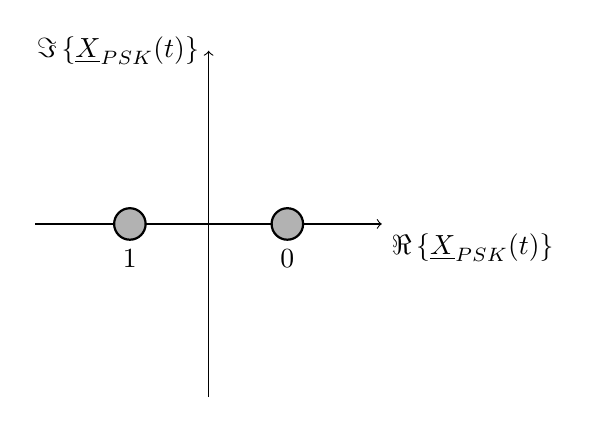
\begin{tikzpicture}
			\draw[->] (-2.2,0) -- (2.2,0) node[below right, align=left]{$\Re\left\{\underline{X}_{PSK}(t)\right\}$};
			\draw[->] (0,-2.2) -- (0,2.2) node[left, align=right]{$\Im\left\{\underline{X}_{PSK}(t)\right\}$};
			
			\draw[black,thick,fill=gray!60] (0:1) ++(0,-0.2) arc(-90:270:0.2) node[below,align=center]{0};
			\draw[black,thick,fill=gray!60] (180:1) ++(0,-0.2) arc(-90:270:0.2) node[below,align=center]{1};
		\end{tikzpicture}
	}

	\caption{\acs{PSK} with $K_m = 2$ discrete states (also known as \ac{BPSK}) capable of encoding 1 bit}
\end{figure}

\begin{figure}[H]
	\centering
	
	\subfloat[\acs{PSK} with $K_m = 4$ in the time-domain]{
		\centering
		\begin{tikzpicture}
			\begin{axis}[
				height={0.15\textheight},
				width=0.35\linewidth,
				scale only axis,
				xlabel={$t$},
				ylabel={$x_{PSK}(t)$},
				%grid style={line width=.6pt, color=lightgray},
				%grid=both,
				grid=none,
				legend pos=outer north east,
				axis y line=middle,
				axis x line=middle,
				every axis x label/.style={
					at={(ticklabel* cs:1.05)},
					anchor=north,
				},
				every axis y label/.style={
					at={(ticklabel* cs:1.05)},
					anchor=east,
				},
				xmin=-0.5,
				xmax=9.5,
				ymin=-1.7,
				ymax=1.7,
				%xtick={0,0.125,...,1},
				%xticklabels={$- \omega_S$, $- \frac{\omega_S}{2}$, $0$, $\frac{\omega_S}{2}$, $\omega_S$},
				%ytick={0},
			]
				\addplot[red, smooth, domain=0:2, samples=50] plot(\x, {cos(deg(2*pi*1*\x))});
				\addplot[red, smooth, domain=2:4, samples=50] plot(\x, {cos(deg(2*pi*1*\x)+270)});
				\addplot[red, smooth, domain=4:6, samples=50] plot(\x, {cos(deg(2*pi*1*\x)+90)});
				\addplot[red, smooth, domain=6:8, samples=50] plot(\x, {cos(deg(2*pi*1*\x)+180)});
				\addplot[red, smooth, domain=8:9, samples=50] plot(\x, {cos(deg(2*pi*1*\x))});
				
				\draw[dashed] (axis cs:2,-1.6) -- (axis cs:2,1.2);
				\draw[dashed] (axis cs:4,-1.6) -- (axis cs:4,1.2);
				\draw[dashed] (axis cs:6,-1.6) -- (axis cs:6,1.2);
				\draw[dashed] (axis cs:8,-1.6) -- (axis cs:8,1.2);
				\draw[latex-latex] (axis cs:4,1.1) -- node[midway,above,align=center]{Symbol period $T_{sym}$} (axis cs:6,1.1);
				
				\draw (1,-1.5) node{0};
				\draw (3,-1.5) node{3};
				\draw (5,-1.5) node{1};
				\draw (7,-1.5) node{2};
			\end{axis}
		\end{tikzpicture}
	}
	\hfill
	\subfloat[Constellation diagram of the \acs{PSK} with $K_m = 4$]{
		\centering
		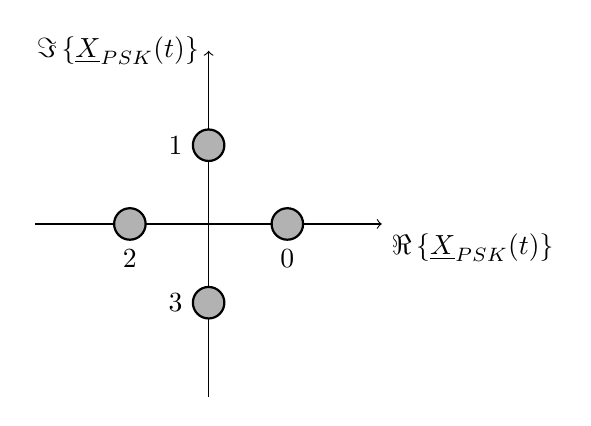
\begin{tikzpicture}
			\draw[->] (-2.2,0) -- (2.2,0) node[below right, align=left]{$\Re\left\{\underline{X}_{PSK}(t)\right\}$};
			\draw[->] (0,-2.2) -- (0,2.2) node[left, align=right]{$\Im\left\{\underline{X}_{PSK}(t)\right\}$};
			
			\draw[black,thick,fill=gray!60] (0:1) ++(0,-0.2) arc(-90:270:0.2) node[below,align=center]{0};
			\draw[black,thick,fill=gray!60] (90:1) ++(-0.2,0) arc(-180:180:0.2) node[left,align=right]{1};
			\draw[black,thick,fill=gray!60] (180:1) ++(0,-0.2) arc(-90:270:0.2) node[below,align=center]{2};
			\draw[black,thick,fill=gray!60] (270:1) ++(-0.2,0) arc(-180:180:0.2) node[left,align=right]{3};
		\end{tikzpicture}
	}
	
	\caption{\acs{PSK} with $K_m = 4$ discrete states (also known as \ac{QPSK}) capable of encoding 2 bit}
\end{figure}

The two examples above depicted the phasor constellations in the complex plane besides the time-domain function of the \ac{PSK} signal.

\begin{definition}{Constellation diagram}
	The \index{symbol constellation} \textbf{symbol constellation} describes all possible phasor values in the complex plane with a symbol associated to it.
	
	The \index{constellation diagram} \textbf{constellation diagram} depicts the symbol constellation graphically.
\end{definition}

\subsection{Quadrature Amplitude Modulation}

Now, \ac{ASK} and \ac{PSK} techniques are combined.
\begin{itemize}
	\item Both amplitude and phase of the carrier are altered.
	\item Using these two dimensions enlarges the set of symbols. Consequently, more data can be transmitted in one symbol.
	\item The modulation is called \index{quadrature amplitude modulation} \textbf{\acf{QAM}}.
	\item The abbreviation \acs{QAM} is often prefixed like \emph{$K_m$-\acs{QAM}}, where $K_m$ is the number of symbols.
	\begin{itemize}
		\item $2$-\acs{QAM} is equivalent to the \ac{BPSK}. The amplitude is constant.
		\item $4$-\acs{QAM} is equivalent to the \ac{QPSK}. The amplitude is constant.
		\item $16$-\acs{QAM} encodes 4 bits in 16 symbols. Both amplitude and phase are used.
		\item $64$-\acs{QAM} encodes 6 bits in 64 symbols. Both amplitude and phase are used.
		\item $256$-\acs{QAM} encodes 8 bits (1 byte) in 256 symbols. Both amplitude and phase are used.
		\item Any other value of can be selected. However, practical implementations only support powers of 2 because binary data (bits) is encoded.
	\end{itemize}
	\item The symbols are distributed with equal spacing to the neighbouring symbols in the complex plane.
\end{itemize}

\begin{fact}
	Because the phase is affected, coherent demodulation is required.
\end{fact}

\begin{figure}[H]
	\centering
	\begin{adjustbox}{scale=1}
		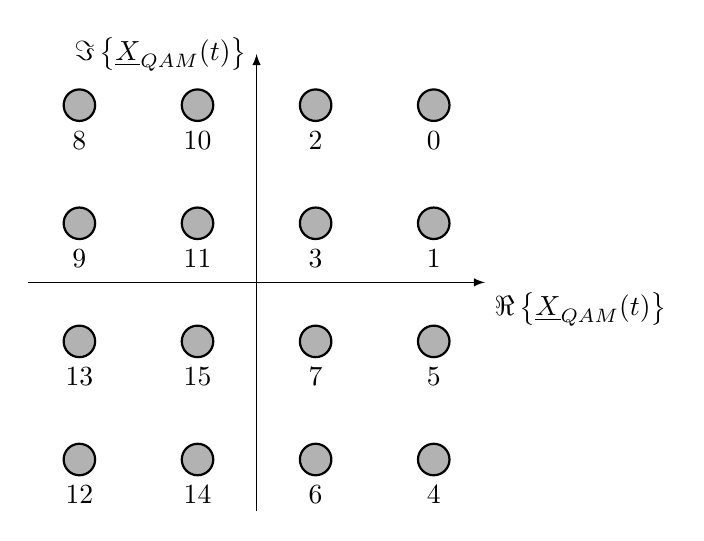
\begin{tikzpicture}[scale=1]
			\draw[-latex] (-2.9,0) -- (2.9,0) node[below right, align=left]{$\Re\left\{\underline{X}_{QAM}(t)\right\}$};
			\draw[-latex] (0,-2.9) -- (0,2.9) node[left, align=right]{$\Im\left\{\underline{X}_{QAM}(t)\right\}$};
			
			\draw[black,thick,fill=gray!60] (2.25,2.25) ++(0,-0.2) arc(-90:270:0.2) node[below,align=center]{0};
			\draw[black,thick,fill=gray!60] (2.25,0.75) ++(0,-0.2) arc(-90:270:0.2) node[below,align=center]{1};
			\draw[black,thick,fill=gray!60] (0.75,2.25) ++(0,-0.2) arc(-90:270:0.2) node[below,align=center]{2};
			\draw[black,thick,fill=gray!60] (0.75,0.75) ++(0,-0.2) arc(-90:270:0.2) node[below,align=center]{3};
			
			\draw[black,thick,fill=gray!60] (2.25,-2.25) ++(0,-0.2) arc(-90:270:0.2) node[below,align=center]{4};
			\draw[black,thick,fill=gray!60] (2.25,-0.75) ++(0,-0.2) arc(-90:270:0.2) node[below,align=center]{5};
			\draw[black,thick,fill=gray!60] (0.75,-2.25) ++(0,-0.2) arc(-90:270:0.2) node[below,align=center]{6};
			\draw[black,thick,fill=gray!60] (0.75,-0.75) ++(0,-0.2) arc(-90:270:0.2) node[below,align=center]{7};
			
			\draw[black,thick,fill=gray!60] (-2.25,2.25) ++(0,-0.2) arc(-90:270:0.2) node[below,align=center]{8};
			\draw[black,thick,fill=gray!60] (-2.25,0.75) ++(0,-0.2) arc(-90:270:0.2) node[below,align=center]{9};
			\draw[black,thick,fill=gray!60] (-0.75,2.25) ++(0,-0.2) arc(-90:270:0.2) node[below,align=center]{10};
			\draw[black,thick,fill=gray!60] (-0.75,0.75) ++(0,-0.2) arc(-90:270:0.2) node[below,align=center]{11};
			
			\draw[black,thick,fill=gray!60] (-2.25,-2.25) ++(0,-0.2) arc(-90:270:0.2) node[below,align=center]{12};
			\draw[black,thick,fill=gray!60] (-2.25,-0.75) ++(0,-0.2) arc(-90:270:0.2) node[below,align=center]{13};
			\draw[black,thick,fill=gray!60] (-0.75,-2.25) ++(0,-0.2) arc(-90:270:0.2) node[below,align=center]{14};
			\draw[black,thick,fill=gray!60] (-0.75,-0.75) ++(0,-0.2) arc(-90:270:0.2) node[below,align=center]{15};
		\end{tikzpicture}
	\end{adjustbox}
	\caption{Example constellation diagram of a $16$-\acs{QAM}}
\end{figure}

\begin{excursus}{Modulation of \ac{QAM} signals}
	The IQ modulator (see Figure \ref{fig:ch05:iq_up_circuit}) can be used to modulate the \ac{QAM} symbols.
	\begin{itemize}
		\item The \underline{real part of the symbol} phasor $\Re\left\{\underline{X}_{PSK}(t)\right\}$ is converted to an analogue signal by a \ac{DAC} and \underline{directly used as the \ac{I} baseband signal}.
		\item The \underline{imaginary part of the symbol} phasor $\Im\left\{\underline{X}_{PSK}(t)\right\}$ is converted to an analogue signal by a \ac{DAC} and \underline{directly used as the \ac{Q} baseband signal}.
	\end{itemize}

	\vspace{0.5em}
	
	The IQ demodulation works vice versa.
\end{excursus}

The number $K_m$ of the $K_m$-\acs{QAM} selects the number of possible symbols in the constellation diagram.
\begin{itemize}
	\item A higher value of $K_m$ enlarges the set of symbols.
	\begin{itemize}
		\item More data can be encoded in one symbol.
		\item The data rate increases while the symbol period is kept constant.
		\item The bandwidth of the transmitted signal remains constant while the data rate increases.
	\end{itemize}
	\item As a drawback, higher values of $K_m$ reduce the noise immunity. Signals need a higher \ac{SNR} to keep the data error after the demodulation low.
	\item Lower values of $K_m$
	\begin{itemize}
		\item are more immune to noise,
		\item are capable of dealing with a poor \ac{SNR} better,
		\item but can encode less data in one symbol, and
		\item therefore have a lower data rate.
	\end{itemize}
\end{itemize}

\begin{excursus}{Signal bandwidth}
	The bandwidth is matters!
	\begin{itemize}
		\item The electromagnetic spectrum is shared with many other applications and services.
		\item \textbf{The electromagnetic spectrum is a sparse resource.}
		\item Its important to use it efficiently. Therefore, each symbol should encode as much data as possible to obtain a high data rate at a moderately narrow bandwidth.
		\item A trade-off must be made between
		\begin{itemize}
			\item a reasonable high value of $K_m$ increasing the data rate and
			\item a reasonable low value of $K_m$ increasing the immunity to noise.
		\end{itemize}
		\item Modern digital communication system are capable of adapting the value of $K_m$ to the current propagation conditions to archive optimal results.
	\end{itemize}
\end{excursus}

\subsection{Inter-Symbol Interference}

\begin{figure}[H]
	\centering
	\begin{tikzpicture}
		\begin{axis}[
			height={0.15\textheight},
			width=0.7\linewidth,
			scale only axis,
			xlabel={$t$},
			ylabel={$x_{sym}(t)$},
			%grid style={line width=.6pt, color=lightgray},
			%grid=both,
			grid=none,
			legend pos=outer north east,
			axis y line=middle,
			axis x line=middle,
			every axis x label/.style={
				at={(ticklabel* cs:1.05)},
				anchor=north,
			},
			every axis y label/.style={
				at={(ticklabel* cs:1.05)},
				anchor=east,
			},
			xmin=-0.5,
			xmax=8.5,
			ymin=0,
			ymax=1.7,
			%xtick={0,0.125,...,1},
			%xticklabels={$- \omega_S$, $- \frac{\omega_S}{2}$, $0$, $\frac{\omega_S}{2}$, $\omega_S$},
			%ytick={0},
		]
			\draw[blue] (axis cs:0,0) -- (axis cs:0,1) -- (axis cs:2,1) -- (axis cs:2,0);
			\draw[red] (axis cs:2,0) -- (axis cs:2,0.55) -- (axis cs:4,0.55) -- (axis cs:4,0);
			\draw[green] (axis cs:4,0) -- (axis cs:4,0.85) -- (axis cs:6,0.85) -- (axis cs:6,0);
			\draw[olive] (axis cs:6,0) -- (axis cs:6,0.7) -- (axis cs:8,0.7) -- (axis cs:8,0);
			
			\draw[dashed] (axis cs:2,0) -- (axis cs:2,1.2);
			\draw[dashed] (axis cs:4,0) -- (axis cs:4,1.2);
			\draw[latex-latex] (axis cs:2,1.1) -- node[midway,above,align=center]{Symbol period $T_{sym}$} (axis cs:4,1.1);
		\end{axis}
	\end{tikzpicture}
	\caption{Series of four ideal symbols}
\end{figure}

\begin{itemize}
	\item \eqref{eq:ch05:sym_rect} defined the symbols as ideal rectangle shapes.
	\item Real implementations this ideal shape does not exist.
	\begin{itemize}
		\item The Fourier transform of the rectangle function is a sinc-function, which indefinitely expands in the frequency domain.
		\item Real system limit the bandwidth. Remember that \acp{LPF} should be applied after mixers and before \ac{ADC}.
	\end{itemize}
	\item Due to the bandwidth-limitation, the rectangle shape is flattened. The ideally steep edges become flattened.
\end{itemize}

\begin{figure}[H]
	\centering
	\begin{tikzpicture}
		\begin{axis}[
			height={0.15\textheight},
			width=0.7\linewidth,
			scale only axis,
			xlabel={$t$},
			ylabel={$x_{sym}(t)$},
			%grid style={line width=.6pt, color=lightgray},
			%grid=both,
			grid=none,
			legend pos=outer north east,
			axis y line=middle,
			axis x line=middle,
			every axis x label/.style={
				at={(ticklabel* cs:1.05)},
				anchor=north,
			},
			every axis y label/.style={
				at={(ticklabel* cs:1.05)},
				anchor=east,
			},
			xmin=-0.5,
			xmax=8.5,
			ymin=0,
			ymax=1.7,
			%xtick={0,0.125,...,1},
			%xticklabels={$- \omega_S$, $- \frac{\omega_S}{2}$, $0$, $\frac{\omega_S}{2}$, $\omega_S$},
			%ytick={0},
		]
			\draw[blue,smooth] (axis cs:-0.25,0) -- (axis cs:0.25,1) -- (axis cs:1.75,1) -- (axis cs:2.25,0);
			\draw[red,smooth] (axis cs:1.75,0) -- (axis cs:2.25,0.55) -- (axis cs:3.75,0.55) -- (axis cs:4.25,0);
			\draw[green,smooth] (axis cs:3.75,0) -- (axis cs:4.25,0.85) -- (axis cs:5.75,0.85) -- (axis cs:6.25,0);
			\draw[olive,smooth] (axis cs:5.75,0) -- (axis cs:6.25,0.7) -- (axis cs:7.75,0.7) -- (axis cs:8.25,0);
			
			\draw[dashed] (axis cs:2,0) -- (axis cs:2,1.2);
			\draw[dashed] (axis cs:4,0) -- (axis cs:4,1.2);
			\draw[latex-latex] (axis cs:2,1.1) -- node[midway,above,align=center]{Symbol period $T_{sym}$} (axis cs:4,1.1);
		\end{axis}
	\end{tikzpicture}
	\caption[Series of four non-ideal symbols showing overlap]{Series of four non-ideal symbols where the edges are flattened. The symbols overlap due to \acs{ISI}.}
\end{figure}

\begin{itemize}
	\item Due to the flattened shape, the symbols overlap.
	\item This effect is the \index{inter-symbol interference} \textbf{\acf{ISI}}.
	\item To mitigate the \ac{ISI} a \index{guard interval} \textbf{guard interval} should be inserted between the symbols.
	\begin{itemize}
		\item The guard interval adds a spacing between the symbol pulses.
		\item The guard interval reduces the \ac{ISI}.
		\item The symbol period is prolonged. It is the sum of the guard interval and the symbol width (which used to equal the symbol period for ideal rectangle shapes)-
	\end{itemize}
	\item Reducing the symbol width by maintaining the symbol period $T_{sym}$ is not feasible, because the bandwidth of the signal would be increased.
\end{itemize}

\begin{figure}[H]
	\centering
	\begin{tikzpicture}
		\begin{axis}[
			height={0.15\textheight},
			width=0.7\linewidth,
			scale only axis,
			xlabel={$t$},
			ylabel={$x_{sym}(t)$},
			%grid style={line width=.6pt, color=lightgray},
			%grid=both,
			grid=none,
			legend pos=outer north east,
			axis y line=middle,
			axis x line=middle,
			every axis x label/.style={
				at={(ticklabel* cs:1.05)},
				anchor=north,
			},
			every axis y label/.style={
				at={(ticklabel* cs:1.05)},
				anchor=east,
			},
			xmin=-0.5,
			xmax=10,
			ymin=0,
			ymax=1.9,
			%xtick={0,0.125,...,1},
			%xticklabels={$- \omega_S$, $- \frac{\omega_S}{2}$, $0$, $\frac{\omega_S}{2}$, $\omega_S$},
			%ytick={0},
		]
			\draw[blue,smooth] (axis cs:-0.25,0) -- (axis cs:0.25,1) -- (axis cs:1.75,1) -- (axis cs:2.25,0);
			\draw[red,smooth] (axis cs:2.25,0) -- (axis cs:2.75,0.55) -- (axis cs:4.25,0.55) -- (axis cs:4.75,0);
			\draw[green,smooth] (axis cs:4.75,0) -- (axis cs:5.25,0.85) -- (axis cs:6.75,0.85) -- (axis cs:7.25,0);
			\draw[olive,smooth] (axis cs:7.25,0) -- (axis cs:7.75,0.7) -- (axis cs:9.25,0.7) -- (axis cs:9.75,0);
			
			\draw[dashed] (axis cs:2.5,0) -- (axis cs:2.5,1.6);
			\draw[dashed] (axis cs:4.5,0) -- (axis cs:4.5,1.4);
			\draw[dashed] (axis cs:5,0) -- (axis cs:5,1.6);
			\draw[latex-latex] (axis cs:2.5,1.5) -- node[midway,above,align=center]{Prolonged symbol period $T_{sym}$} (axis cs:5,1.5);
			\draw[latex-latex] (axis cs:2.5,1.3) node[left,align=right]{Symbol width} -- (axis cs:4.5,1.3);
			\draw[latex-latex] (axis cs:4.5,1.3) -- (axis cs:5,1.3) node[right,align=left]{Guard interval};
		\end{axis}
	\end{tikzpicture}
	\caption[Series of four non-ideal symbols with additional spacing]{Series of four non-ideal symbols where the edges are flattened. An additional spacing between the symbols (guard interval) is added to mitigate \acs{ISI}. The symbol period is prolonged by the guard interval.}
\end{figure}

\subsection{IQ Imbalance}

So far, we assumed ideal conditions for the IQ modulation and IQ demodulation (see Figure \ref{fig:ch05:iq_up_circuit} and \ref{fig:ch05:iq_down_circuit}).
\begin{itemize}
	\item The phase-shift of the \ac{LO} signal was perfectly \SI{90}{\degree}.
	\item The phasor of the \ac{LO} signal fed into the \ac{I}-mixer was ideally parallel to the real axis in the complex plane ($\arg\left(\underline{X}_{LO,I}\right) = 0$).
	\item The phasor of the phase-shifted \ac{LO} signal fed into the \ac{Q}-mixer was ideally parallel to the imaginary axis in the complex plane ($\arg\left(\underline{X}_{LO,Q}\right) = \frac{\pi}{2}$).
	\item Both phasors were perfectly orthogonal.
\end{itemize}

\begin{figure}[H]
	\centering
	
	\subfloat[Example constellation diagram of a $16$-\acs{QAM} under ideal conditions]{
		\centering
		\begin{adjustbox}{scale=0.9}
			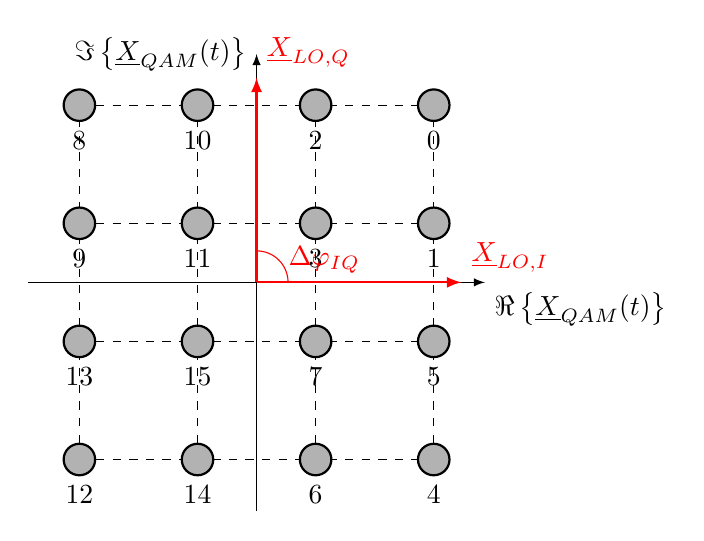
\begin{tikzpicture}[scale=1]
				\draw[-latex] (-2.9,0) -- (2.9,0) node[below right, align=left]{$\Re\left\{\underline{X}_{QAM}(t)\right\}$};
				\draw[-latex] (0,-2.9) -- (0,2.9) node[left, align=right]{$\Im\left\{\underline{X}_{QAM}(t)\right\}$};
				
				\pgftransformcm{1}{0}{0}{1}{\pgfpoint{0cm}{0cm}}
				
				\foreach \x in {-2.25,-0.75,0.75,2.25}{
					\draw[dashed] (\x,-2.25) -- (\x,2.25);
					\draw[dashed] (-2.25,\x) -- (2.25,\x);
				}
				
				
				\draw[black,thick,fill=gray!60] (2.25,2.25) ++(0,-0.2) arc(-90:270:0.2) node[below,align=center]{0};
				\draw[black,thick,fill=gray!60] (2.25,0.75) ++(0,-0.2) arc(-90:270:0.2) node[below,align=center]{1};
				\draw[black,thick,fill=gray!60] (0.75,2.25) ++(0,-0.2) arc(-90:270:0.2) node[below,align=center]{2};
				\draw[black,thick,fill=gray!60] (0.75,0.75) ++(0,-0.2) arc(-90:270:0.2) node[below,align=center]{3};
				
				\draw[black,thick,fill=gray!60] (2.25,-2.25) ++(0,-0.2) arc(-90:270:0.2) node[below,align=center]{4};
				\draw[black,thick,fill=gray!60] (2.25,-0.75) ++(0,-0.2) arc(-90:270:0.2) node[below,align=center]{5};
				\draw[black,thick,fill=gray!60] (0.75,-2.25) ++(0,-0.2) arc(-90:270:0.2) node[below,align=center]{6};
				\draw[black,thick,fill=gray!60] (0.75,-0.75) ++(0,-0.2) arc(-90:270:0.2) node[below,align=center]{7};
				
				\draw[black,thick,fill=gray!60] (-2.25,2.25) ++(0,-0.2) arc(-90:270:0.2) node[below,align=center]{8};
				\draw[black,thick,fill=gray!60] (-2.25,0.75) ++(0,-0.2) arc(-90:270:0.2) node[below,align=center]{9};
				\draw[black,thick,fill=gray!60] (-0.75,2.25) ++(0,-0.2) arc(-90:270:0.2) node[below,align=center]{10};
				\draw[black,thick,fill=gray!60] (-0.75,0.75) ++(0,-0.2) arc(-90:270:0.2) node[below,align=center]{11};
				
				\draw[black,thick,fill=gray!60] (-2.25,-2.25) ++(0,-0.2) arc(-90:270:0.2) node[below,align=center]{12};
				\draw[black,thick,fill=gray!60] (-2.25,-0.75) ++(0,-0.2) arc(-90:270:0.2) node[below,align=center]{13};
				\draw[black,thick,fill=gray!60] (-0.75,-2.25) ++(0,-0.2) arc(-90:270:0.2) node[below,align=center]{14};
				\draw[black,thick,fill=gray!60] (-0.75,-0.75) ++(0,-0.2) arc(-90:270:0.2) node[below,align=center]{15};
				
				\draw[-latex,red,thick] (0,0) -- (2.6,0) node[above right, align=left]{$\underline{X}_{LO,I}$};
				\draw[-latex,red,thick] (0,0) -- (0,2.6) node[above right, align=left]{$\underline{X}_{LO,Q}$};
				\draw[red] (0:0.4) arc(0:90:0.4) node[midway,right,align=left]{$\Delta \varphi_{IQ}$};
			\end{tikzpicture}
		\end{adjustbox}
	}
	\hfill
	\subfloat[Example constellation diagram of a $16$-\acs{QAM} subject to IQ imbalance]{
		\centering
		\begin{adjustbox}{scale=0.9}
			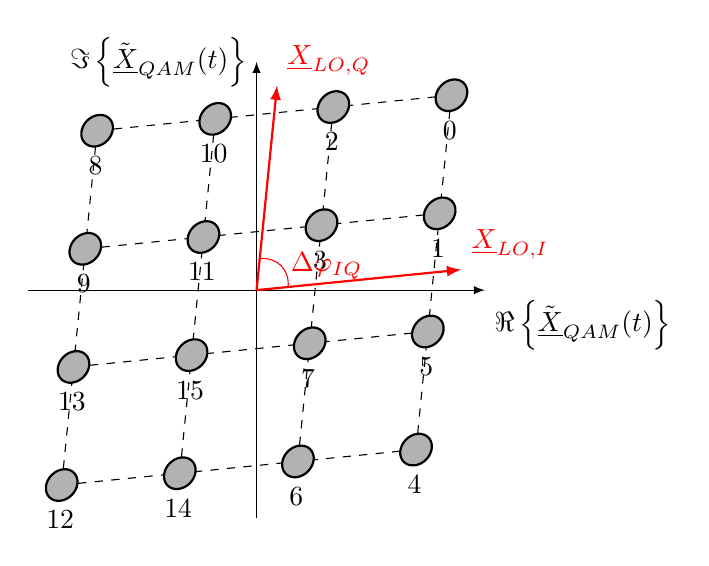
\begin{tikzpicture}[scale=1]
				\draw[-latex] (-2.9,0) -- (2.9,0) node[below right, align=left]{$\Re\left\{\tilde{\underline{X}}_{QAM}(t)\right\}$};
				\draw[-latex] (0,-2.9) -- (0,2.9) node[left, align=right]{$\Im\left\{\tilde{\underline{X}}_{QAM}(t)\right\}$};
				
				\pgftransformcm{1}{0.1}{0.1}{1}{\pgfpoint{0cm}{0cm}}
				
				\foreach \x in {-2.25,-0.75,0.75,2.25}{
					\draw[dashed] (\x,-2.25) -- (\x,2.25);
					\draw[dashed] (-2.25,\x) -- (2.25,\x);
				}
				
				
				\draw[black,thick,fill=gray!60] (2.25,2.25) ++(0,-0.2) arc(-90:270:0.2) node[below,align=center]{0};
				\draw[black,thick,fill=gray!60] (2.25,0.75) ++(0,-0.2) arc(-90:270:0.2) node[below,align=center]{1};
				\draw[black,thick,fill=gray!60] (0.75,2.25) ++(0,-0.2) arc(-90:270:0.2) node[below,align=center]{2};
				\draw[black,thick,fill=gray!60] (0.75,0.75) ++(0,-0.2) arc(-90:270:0.2) node[below,align=center]{3};
				
				\draw[black,thick,fill=gray!60] (2.25,-2.25) ++(0,-0.2) arc(-90:270:0.2) node[below,align=center]{4};
				\draw[black,thick,fill=gray!60] (2.25,-0.75) ++(0,-0.2) arc(-90:270:0.2) node[below,align=center]{5};
				\draw[black,thick,fill=gray!60] (0.75,-2.25) ++(0,-0.2) arc(-90:270:0.2) node[below,align=center]{6};
				\draw[black,thick,fill=gray!60] (0.75,-0.75) ++(0,-0.2) arc(-90:270:0.2) node[below,align=center]{7};
				
				\draw[black,thick,fill=gray!60] (-2.25,2.25) ++(0,-0.2) arc(-90:270:0.2) node[below,align=center]{8};
				\draw[black,thick,fill=gray!60] (-2.25,0.75) ++(0,-0.2) arc(-90:270:0.2) node[below,align=center]{9};
				\draw[black,thick,fill=gray!60] (-0.75,2.25) ++(0,-0.2) arc(-90:270:0.2) node[below,align=center]{10};
				\draw[black,thick,fill=gray!60] (-0.75,0.75) ++(0,-0.2) arc(-90:270:0.2) node[below,align=center]{11};
				
				\draw[black,thick,fill=gray!60] (-2.25,-2.25) ++(0,-0.2) arc(-90:270:0.2) node[below,align=center]{12};
				\draw[black,thick,fill=gray!60] (-2.25,-0.75) ++(0,-0.2) arc(-90:270:0.2) node[below,align=center]{13};
				\draw[black,thick,fill=gray!60] (-0.75,-2.25) ++(0,-0.2) arc(-90:270:0.2) node[below,align=center]{14};
				\draw[black,thick,fill=gray!60] (-0.75,-0.75) ++(0,-0.2) arc(-90:270:0.2) node[below,align=center]{15};
				
				\draw[-latex,red,thick] (0,0) -- (2.6,0) node[above right, align=left]{$\underline{X}_{LO,I}$};
				\draw[-latex,red,thick] (0,0) -- (0,2.6) node[above right, align=left]{$\underline{X}_{LO,Q}$};
				\draw[red] (0:0.4) arc(0:90:0.4) node[midway,right,align=left]{$\Delta \varphi_{IQ}$};
			\end{tikzpicture}
		\end{adjustbox}
	}

	\caption{Example constellation diagram of a $16$-\acs{QAM} under ideal conditions and while being subject to IQ imbalance}
\end{figure}

Under real conditions, the phase-shift of the \ac{LO} signal is not precisely \SI{90}{\degree}.
\begin{itemize}
	\item The phase-shift between the \ac{I} and \ac{Q} component of the \ac{LO} signal $\Delta \varphi_{IQ}$ differs from \SI{90}{\degree}.
	\item The difference $\SI{90}{\degree} - \Delta \varphi_{IQ}$ is the \index{IQ imbalance} \textbf{IQ imbalance}.
	\item The IQ imbalance will disturb the data detection, which reconstructs the symbols from the IQ demodulated \ac{I} and \ac{Q} baseband signals.
	\item Data error might a corollary of the IQ imbalance.
\end{itemize}

Countermeasures:
\begin{itemize}
	\item The IQ imbalance is a linear coordinate transformation.
	\begin{equation}
		\underbrace{\left[\begin{matrix}\Re\left\{\tilde{\underline{X}}_{QAM}(t)\right\}\\ \Im\left\{\tilde{\underline{X}}_{QAM}(t)\right\}\end{matrix}\right]}_{\text{IQ imbalance applied}} = \mat{T}_{IQ} \cdot \underbrace{\left[\begin{matrix}\Re\left\{\underline{X}_{QAM}(t)\right\}\\ \Im\left\{\underline{X}_{QAM}(t)\right\}\end{matrix}\right]}_{\text{Ideal constellation}}
	\end{equation}
	where $\mat{T}_{IQ}$ is a $2 \times 2$ transformation matrix.
	\item The IQ imbalance must be estimated to obtain knowledge about $\mat{T}_{IQ}$.
	\item The IQ imbalance can then be compensated by applying the inverse transformation matrix $\mat{T}_{IQ}^{-1}$.
\end{itemize}

\subsection{Synchronization 2: Carrier Recovery}

\subsubsection{Phase Offset}

Another problem is that the phase of the \ac{RF} signal is not known.
\begin{itemize}
	\item The phases of the transmitter \ac{LO} and the receiver \ac{LO} are not synchronized.
	\item They are phase-shifted by a \emph{phase offset} of $\Delta \varphi_{C}$ (``C'' stands for carrier).
	\item A corollary is that the \ac{RF} carrier, which is synchronous to the transmitter \ac{LO}, is phase-shifted by $\Delta \varphi_{C}$ in relation to the receiver \ac{LO}.
	\item The whole constellation diagram is rotated by $\Delta \varphi_{C}$.
\end{itemize}

\textit{The IQ imbalance is neglected for the following considerations.}

\begin{figure}[H]
	\centering
	\begin{adjustbox}{scale=1}
		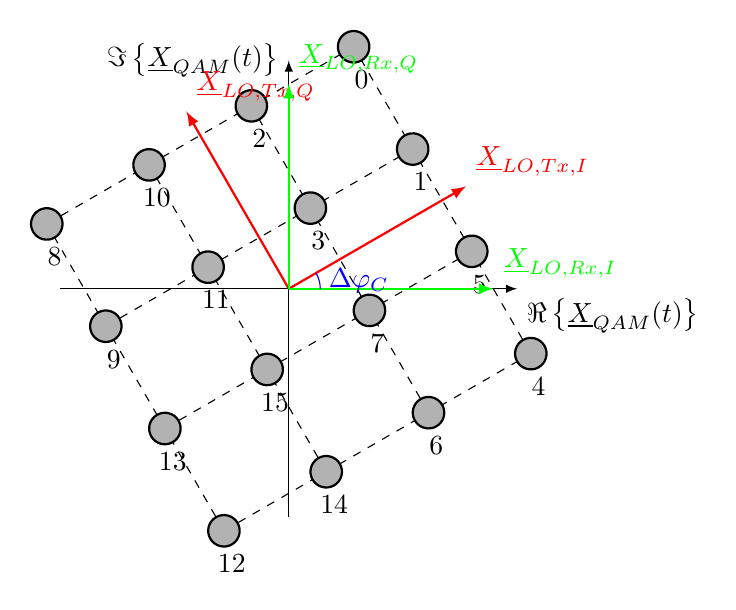
\begin{tikzpicture}[scale=1]
			\draw[-latex] (-2.9,0) -- (2.9,0) node[below right, align=left]{$\Re\left\{\underline{X}_{QAM}(t)\right\}$};
			\draw[-latex] (0,-2.9) -- (0,2.9) node[left, align=right]{$\Im\left\{\underline{X}_{QAM}(t)\right\}$};
			
			\begin{scope}[rotate=30]
				\foreach \x in {-2.25,-0.75,0.75,2.25}{
					\draw[dashed] (\x,-2.25) -- (\x,2.25);
					\draw[dashed] (-2.25,\x) -- (2.25,\x);
				}
		
				\draw[black,thick,fill=gray!60] (2.25,2.25) ++(0,-0.2) arc(-90:270:0.2) node[below,align=center]{0};
				\draw[black,thick,fill=gray!60] (2.25,0.75) ++(0,-0.2) arc(-90:270:0.2) node[below,align=center]{1};
				\draw[black,thick,fill=gray!60] (0.75,2.25) ++(0,-0.2) arc(-90:270:0.2) node[below,align=center]{2};
				\draw[black,thick,fill=gray!60] (0.75,0.75) ++(0,-0.2) arc(-90:270:0.2) node[below,align=center]{3};
				
				\draw[black,thick,fill=gray!60] (2.25,-2.25) ++(0,-0.2) arc(-90:270:0.2) node[below,align=center]{4};
				\draw[black,thick,fill=gray!60] (2.25,-0.75) ++(0,-0.2) arc(-90:270:0.2) node[below,align=center]{5};
				\draw[black,thick,fill=gray!60] (0.75,-2.25) ++(0,-0.2) arc(-90:270:0.2) node[below,align=center]{6};
				\draw[black,thick,fill=gray!60] (0.75,-0.75) ++(0,-0.2) arc(-90:270:0.2) node[below,align=center]{7};
				
				\draw[black,thick,fill=gray!60] (-2.25,2.25) ++(0,-0.2) arc(-90:270:0.2) node[below,align=center]{8};
				\draw[black,thick,fill=gray!60] (-2.25,0.75) ++(0,-0.2) arc(-90:270:0.2) node[below,align=center]{9};
				\draw[black,thick,fill=gray!60] (-0.75,2.25) ++(0,-0.2) arc(-90:270:0.2) node[below,align=center]{10};
				\draw[black,thick,fill=gray!60] (-0.75,0.75) ++(0,-0.2) arc(-90:270:0.2) node[below,align=center]{11};
				
				\draw[black,thick,fill=gray!60] (-2.25,-2.25) ++(0,-0.2) arc(-90:270:0.2) node[below,align=center]{12};
				\draw[black,thick,fill=gray!60] (-2.25,-0.75) ++(0,-0.2) arc(-90:270:0.2) node[below,align=center]{13};
				\draw[black,thick,fill=gray!60] (-0.75,-2.25) ++(0,-0.2) arc(-90:270:0.2) node[below,align=center]{14};
				\draw[black,thick,fill=gray!60] (-0.75,-0.75) ++(0,-0.2) arc(-90:270:0.2) node[below,align=center]{15};
				
				\draw[-latex,red,thick] (0,0) -- (2.6,0) node[above right, align=left]{$\underline{X}_{LO,Tx,I}$};
				\draw[-latex,red,thick] (0,0) -- (0,2.6) node[above right, align=left]{$\underline{X}_{LO,Tx,Q}$};
			\end{scope}
			
			\draw[-latex,green,thick] (0,0) -- (2.6,0) node[above right, align=left]{$\underline{X}_{LO,Rx,I}$};
			\draw[-latex,green,thick] (0,0) -- (0,2.6) node[above right, align=left]{$\underline{X}_{LO,Rx,Q}$};
			
			\draw[blue] (0:0.4) arc(0:30:0.4) node[midway,right,align=left]{$\Delta \varphi_{C}$};
		\end{tikzpicture}
	\end{adjustbox}
	\caption{Example constellation diagram of a $16$-\acs{QAM} rotated by a phase offset of $\Delta \varphi_{C} = \SI{30}{\degree}$}
\end{figure}

\textbf{The data detection will fail, because the detector expects a perfectly adjusted symbol constellation.}

\subsubsection{Frequency Offset}

In addition to the phase offset, the frequency of the transmitter \ac{LO} and receiver \ac{LO} might differ.
\begin{itemize}
	\item The difference is the \emph{frequency offset} $\Delta \omega_{C}$.
	\item The \ac{RF} carrier is synchronized to the transmitter \ac{LO}. Its frequency differs by $\Delta \omega_{C}$ from the receiver \ac{LO}.
	\item A corollary is that the phase offset integrates over time.
	\begin{equation}
		\Delta \varphi_{C}(t) = \underbrace{\Delta \varphi_{C,0}}_{\text{Initial offset}} + \int\limits_{t_0}^{t} \omega_{C} \, \mathrm{d} t
	\end{equation}
	\item The constellation diagram rotates at $\omega_{C}$ and constantly changes its angle.
\end{itemize}

\begin{figure}[H]
	\centering
	\begin{adjustbox}{scale=1}
		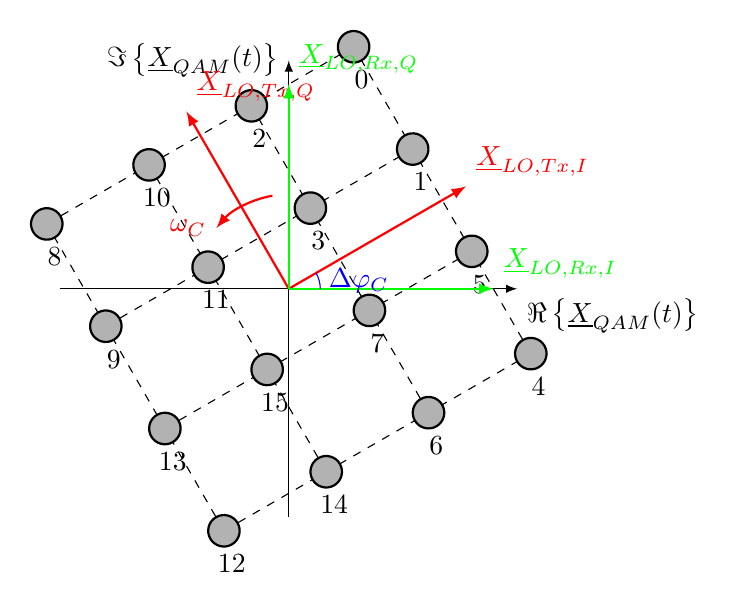
\begin{tikzpicture}[scale=1]
			\draw[-latex] (-2.9,0) -- (2.9,0) node[below right, align=left]{$\Re\left\{\underline{X}_{QAM}(t)\right\}$};
			\draw[-latex] (0,-2.9) -- (0,2.9) node[left, align=right]{$\Im\left\{\underline{X}_{QAM}(t)\right\}$};
			
			\begin{scope}[rotate=30]
				\foreach \x in {-2.25,-0.75,0.75,2.25}{
					\draw[dashed] (\x,-2.25) -- (\x,2.25);
					\draw[dashed] (-2.25,\x) -- (2.25,\x);
				}
				
				\draw[black,thick,fill=gray!60] (2.25,2.25) ++(0,-0.2) arc(-90:270:0.2) node[below,align=center]{0};
				\draw[black,thick,fill=gray!60] (2.25,0.75) ++(0,-0.2) arc(-90:270:0.2) node[below,align=center]{1};
				\draw[black,thick,fill=gray!60] (0.75,2.25) ++(0,-0.2) arc(-90:270:0.2) node[below,align=center]{2};
				\draw[black,thick,fill=gray!60] (0.75,0.75) ++(0,-0.2) arc(-90:270:0.2) node[below,align=center]{3};
				
				\draw[black,thick,fill=gray!60] (2.25,-2.25) ++(0,-0.2) arc(-90:270:0.2) node[below,align=center]{4};
				\draw[black,thick,fill=gray!60] (2.25,-0.75) ++(0,-0.2) arc(-90:270:0.2) node[below,align=center]{5};
				\draw[black,thick,fill=gray!60] (0.75,-2.25) ++(0,-0.2) arc(-90:270:0.2) node[below,align=center]{6};
				\draw[black,thick,fill=gray!60] (0.75,-0.75) ++(0,-0.2) arc(-90:270:0.2) node[below,align=center]{7};
				
				\draw[black,thick,fill=gray!60] (-2.25,2.25) ++(0,-0.2) arc(-90:270:0.2) node[below,align=center]{8};
				\draw[black,thick,fill=gray!60] (-2.25,0.75) ++(0,-0.2) arc(-90:270:0.2) node[below,align=center]{9};
				\draw[black,thick,fill=gray!60] (-0.75,2.25) ++(0,-0.2) arc(-90:270:0.2) node[below,align=center]{10};
				\draw[black,thick,fill=gray!60] (-0.75,0.75) ++(0,-0.2) arc(-90:270:0.2) node[below,align=center]{11};
				
				\draw[black,thick,fill=gray!60] (-2.25,-2.25) ++(0,-0.2) arc(-90:270:0.2) node[below,align=center]{12};
				\draw[black,thick,fill=gray!60] (-2.25,-0.75) ++(0,-0.2) arc(-90:270:0.2) node[below,align=center]{13};
				\draw[black,thick,fill=gray!60] (-0.75,-2.25) ++(0,-0.2) arc(-90:270:0.2) node[below,align=center]{14};
				\draw[black,thick,fill=gray!60] (-0.75,-0.75) ++(0,-0.2) arc(-90:270:0.2) node[below,align=center]{15};
				
				\draw[-latex,red,thick] (0,0) -- (2.6,0) node[above right, align=left]{$\underline{X}_{LO,Tx,I}$};
				\draw[-latex,red,thick] (0,0) -- (0,2.6) node[above right, align=left]{$\underline{X}_{LO,Tx,Q}$};
				
				\draw[-latex,red,thick] (70:1.2) arc(70:110:1.2) node[left, align=right]{$\omega_{C}$};
			\end{scope}
			
			\draw[-latex,green,thick] (0,0) -- (2.6,0) node[above right, align=left]{$\underline{X}_{LO,Rx,I}$};
			\draw[-latex,green,thick] (0,0) -- (0,2.6) node[above right, align=left]{$\underline{X}_{LO,Rx,Q}$};
			
			\draw[blue] (0:0.4) arc(0:30:0.4) node[midway,right,align=left]{$\Delta \varphi_{C}$};
		\end{tikzpicture}
	\end{adjustbox}
	\caption{Example constellation diagram of a $16$-\acs{QAM} rotating at a frequency offset of $\Delta \omega_{C}$}
\end{figure}

\textbf{The frequency offset and the rotation symbol constellation makes a data detection impossible.}

\subsubsection{Carrier Recovery}

\begin{fact}
	The receiver \ac{LO} must be synchronized to the \ac{RF} carrier phase and frequency.
\end{fact}

The synchronization is called \index{carrier recovery} \textbf{carrier recovery} and is usually implemented as a closed control loop.
\begin{itemize}
	\item The control loop adjusts the \ac{LO} phase so that it is synchronous to the \ac{RF} carrier ($\Delta \omega_{C} \rightarrow 0$).
	\item A synchronization usually requires data (pilot, preamble) to estimate the phase offset from the current symbol constellation.
	\item The phase offset correction is usually sufficient, because the frequency offset is related to that error via the integral. Because of the frequency offset, the synchronization is only short-term stable and must be repeated regularly.
	\item The estimated phase error is than fed via a loop filter to the \ac{LO} (hybrid approach).
	\item An alternative approach is all-digital: The digital \ac{I} and \ac{Q} signals are digitally mixed to compensate the phase and frequency offset.
\end{itemize}

\textit{Remark:} In contrast to the similar timing recovery, which adjusts the sampling clock, the carrier recovery adjusts the \ac{LO}.

\begin{figure}[H]
	\centering
	\begin{adjustbox}{scale=0.6}
		\begin{circuitikz}
			\node[draw, block] at(0,0) (Mixer){Mixer};
			\node[oscillator, below=4cm of Mixer](LO){};
			\node[draw, block, right=of Mixer](Sampler){Sampler};
			\node[oscillator, below=of Sampler](Clock){};
			\node[draw, block, right=of Clock] (Filter){Loop filter};
			\node[draw, block, right=of Filter] (Pred){Timing error\\ estimator};
			\node[draw, block, right=5cm of LO] (CarrierFilter){Loop filter};
			\node[draw, block, right=of CarrierFilter] (CarrierPred){Phase error\\ estimator};
			
			\draw[dashed] (Sampler.north) -- ++(0, 2cm) node[below left, align=right]{Analogue\\ domain} node[below right, align=left]{Digital\\ domain};
			\node[left=2mm of LO, align=right]{\acs{LO}};
			\node[left=2mm of Clock, align=right]{Sampling\\ clock};
			
			\draw[o->] (-2.5,0) node[left,align=right]{Input} -- (Mixer.west);
			\draw[->] (Mixer.east) -- (Sampler.west);
			\draw[->] (Sampler.east) -- ++(11,0) node[right,align=left]{Further signal\\ processing};
			
			\draw[*->] ([xshift=9cm] Sampler.east) |- (Pred.east);
			\draw[->] (Pred.west) -- (Filter.east);
			\draw[->] (Filter.west) -- (Clock.east);
			
			\draw[*->] ([xshift=9.5cm] Sampler.east) |- (CarrierPred.east);
			\draw[->] (CarrierPred.west) -- (CarrierFilter.east);
			\draw[->] (CarrierFilter.west) -- (LO.east);
			
			\draw[->] (LO.north) -- (Mixer.south);
			\draw[->] (Clock.north) -- (Sampler.south);
		\end{circuitikz}
	\end{adjustbox}
	\caption{Hybrid timing recovery and carrier recovery}
\end{figure}

\begin{figure}[H]
	\centering
	\begin{adjustbox}{scale=0.6}
		\begin{circuitikz}
			\node[draw, block] at(0,0) (Mixer){Mixer};
			\node[oscillator, below=3cm of Mixer](LO){};
			\node[draw, block, right=of Mixer](Sampler){Sampler};
			\node[oscillator, below=of Sampler](Clock){};
			\node[draw, block, right=of Sampler] (DigiMix){Digital\\ mixer};
			\node[oscillator, below=4.5cm of DigiMix](NCO){};
			\node[draw, block, right=of DigiMix] (Resampler){Interpolation\\ and resampling};
			\node[draw, block, below=of Resampler] (Filter){Loop filter};
			\node[draw, block, right=of Filter] (Pred){Timing error\\ estimator};
			\node[draw, block, right=of NCO] (CarrierFilter){Loop filter};
			\node[draw, block, right=of CarrierFilter] (CarrierPred){Phase error\\ estimator};
			
			\draw[dashed] (Sampler.north) -- ++(0, 2cm) node[below left, align=right]{Analogue\\ domain} node[below right, align=left]{Digital\\ domain};
			\node[below=2mm of LO, align=center]{Free-running\\ \acs{LO}};
			\node[below=2mm of Clock, align=center]{Free-running\\ sampling clock};
			\node[left=2mm of NCO, align=right]{Digital\\ oscillator};
			
			\draw[o->] (-2.5,0) node[left,align=right]{Input} -- (Mixer.west);
			\draw[->] (Mixer.east) -- (Sampler.west);
			\draw[->] (Sampler.east) -- (DigiMix.west);
			\draw[->] (DigiMix.east) -- (Resampler.west);
			\draw[->] (Resampler.east) -- ++(6,0) node[right,align=left]{Further signal\\ processing};
			
			\draw[*->] ([xshift=5cm] Resampler.east) |- (Pred.east);
			\draw[->] (Pred.west) -- (Filter.east);
			\draw[->] (Filter.north) -- (Resampler.south);
			
			\draw[*->] ([xshift=5.5cm] Resampler.east) |- (CarrierPred.east);
			\draw[->] (CarrierPred.west) -- (CarrierFilter.east);
			\draw[->] (CarrierFilter.west) -- (NCO.east);
			
			\draw[->] (LO.north) -- (Mixer.south);
			\draw[->] (Clock.north) -- (Sampler.south);
			\draw[->] (NCO.north) -- (DigiMix.south);
		\end{circuitikz}
	\end{adjustbox}
	\caption{Digital timing recovery and carrier recovery}
\end{figure}


\phantomsection
\addcontentsline{toc}{section}{References}
\printbibliography[heading=subbibliography]
\end{refsection}

